\thispagestyle{toancuabinone}
\pagestyle{toancuabi}
\everymath{\color{toancuabi}}
%\blfootnote{$^1$\color{toancuabi}Đại học Thăng Long.}
\graphicspath{{../toancuabi/pic/}}
\begingroup
\AddToShipoutPicture*{\put(0,616){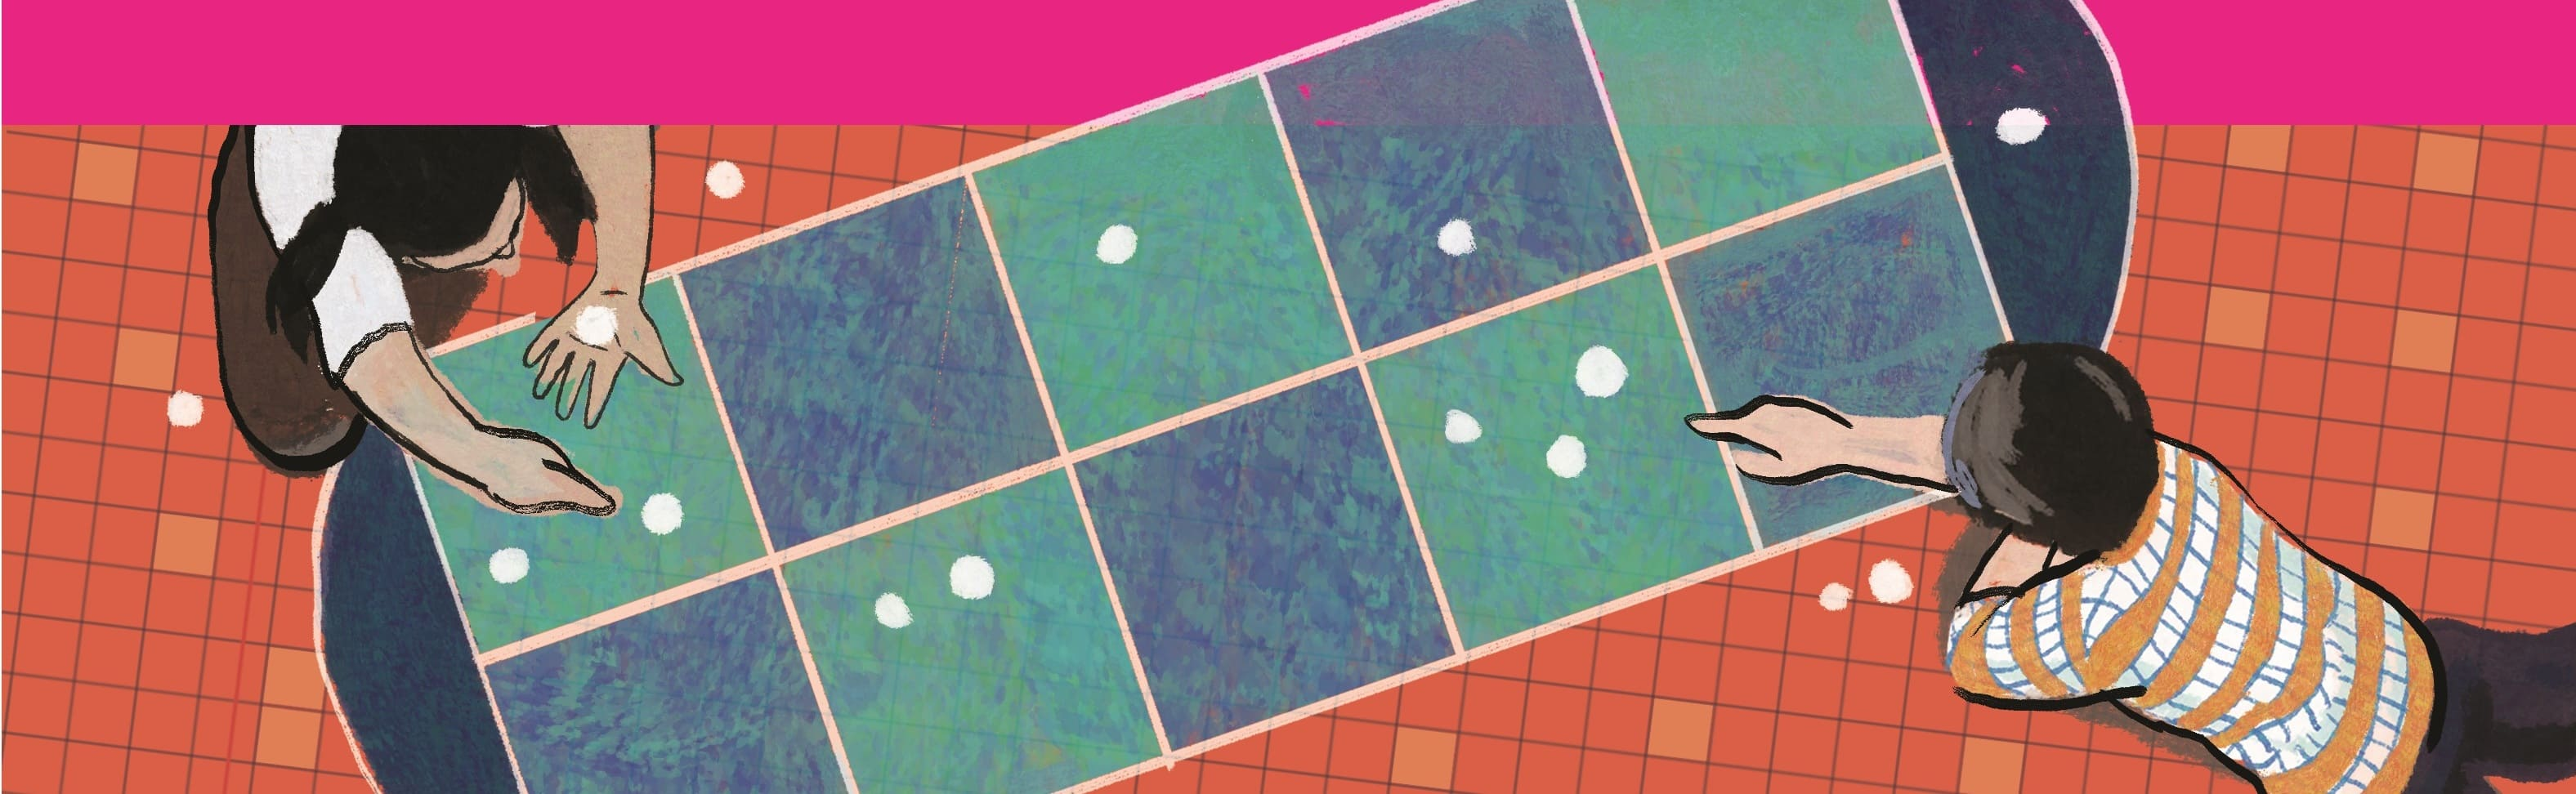
\includegraphics[width=19.3cm]{../bannertoancuabi}}}  
\AddToShipoutPicture*{\put(85,525){
\includegraphics[scale=1]{../tieude1.pdf}}} 
\centering
\endgroup

\vspace*{180pt}

\begin{multicols}{2}
	Mục Toán của Bi trong Số $11$, Tập $6$ đã giới thiệu đến các em cách tính diện tích của những hình tạo trên lưới ô vuông. Rất nhiều hình khác nhau có các đỉnh tại các điểm nguyên đều tính được mà chỉ cần dựa trên những ô vuông đơn vị có diện tích $1$. Không biết diện tích của những hình trên lưới có liên hệ gì với những điểm trên lưới không nhỉ? Định lý Pick được giới thiệu trong phần này sẽ trả lời cho ta câu hỏi rất thú vị này đấy.
	\vskip 0.1cm
	$\pmb{1.}$ \textbf{\color{toancuabi}Định lý Pick}
	\vskip 0.1cm
	Để xem diện tích của một hình trên lưới tính thế nào qua các điểm trên lưới (còn gọi là điểm nguyên), chúng ta thử tính diện tích của một hình cơ bản trong Phần $1$ -- hình chữ nhật kích thước $3\times4$ có các cạnh nằm trên các đường thẳng của lưới bằng một cách khác nhé. Bây giờ, ta chia hình chữ nhật đã cho bởi những đường thẳng song song, cách đều, đi qua giữa hai điểm nguyên trên các cạnh của hình chữ nhật như trong Hình $1$ dưới đây. 
	\begin{figure}[H]
		\vspace*{-5pt}
		\centering
		\captionsetup{labelformat= empty, justification=centering}
		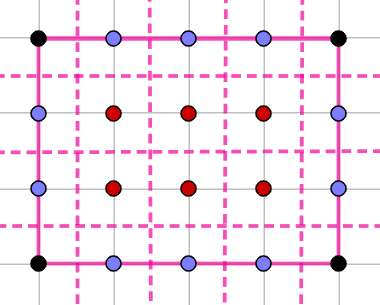
\includegraphics[width= 0.62\linewidth]{1}
		\caption{\small\textit{\color{toancuabi}Hình $1$.}}
		\vspace*{-5pt}
	\end{figure}
	Khi đó ta thấy
	\vskip 0.1cm
	-- Mỗi điểm nguyên ({\color{red}màu đỏ}) nằm trong hình chữ nhật ứng với một hình vuông đơn vị;
	\vskip 0.1cm
	-- Mỗi điểm nguyên ({\color{blue}màu xanh dương}) nằm trên các cạnh của hình chữ nhật mà không phải đỉnh ứng với một nửa hình vuông đơn vị;
	\vskip 0.1cm
	Mỗi điểm nguyên là đỉnh ({\color{black}màu đen}) của hình chữ nhật ứng với một phần tư hình vuông đơn vị.
	\vskip 0.1cm
	Như vậy
	\vskip 0.1cm
	Diện tích của hình chữ nhật $=$ số điểm trong hình chữ nhật
	$+ \dfrac{1}{2}\times$ số điểm trên cạnh mà không phải đỉnh $+ \dfrac{1}{4}\times$ số đỉnh
	\vskip 0.1cm
	Do hình chữ nhật có $4$ đỉnh nên ta thấy ngay
	\vskip 0.1cm
	Diện tích của hình chữ nhật $=$ số điểm trong hình chữ nhật 
	$+ \dfrac{1}{2} \times$ số điểm nằm trên cạnh
	$- 1$.
	\vskip 0.1cm
	Từ đó ta có diện tích của hình chữ nhật trên là:
	\begin{align*}
		6 + \frac{1}{2}\times14 - 1 = 12 \text{ (đơn vị diện tích).}
	\end{align*}
	Ví dụ trên được tính trong một trường hợp cụ thể, tuy nhiên những lập luận này hoàn toàn có thể áp dụng cho tất cả những hình chữ nhật khác cùng đặc điểm. Như vậy diện tích của hình chữ nhật có các cạnh trùng với những đường thẳng của lưới có thể được tính thông qua số điểm nguyên nằm trong và nằm trên cạnh của hình chữ nhật. Nếu ta gọi $T$ là số điểm nằm trong và $B$ là số điểm nằm trên các cạnh của hình chữ nhật, thì diện tích của hình chữ nhật là:
	\begin{align*}
		T+  \frac{B}{2} - 1.
	\end{align*}
	Một công thức thật đơn giản, thật hay đúng không các em. Không biết ngoài hình chữ nhật, công thức tính diện tích này còn đúng với những hình nào nữa nhỉ?
	\vskip 0.1cm
	Chúng ta cùng xem xét diện tích hình cơ bản thứ hai được đề cập trong Phần $1$ -- tam giác vuông có hai cạnh góc vuông trùng với những đường thẳng của lưới.
	\begin{figure}[H]
		\vspace*{-5pt}
		\centering
		\captionsetup{labelformat= empty, justification=centering}
		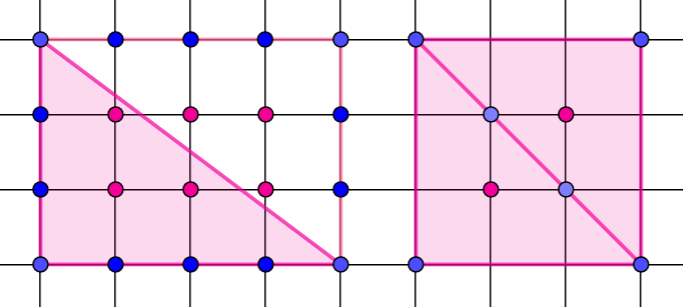
\includegraphics[width= 0.7\linewidth]{2}
		\caption{\small\textit{\color{toancuabi}Hình $2$.}}
		\vspace*{-10pt}
	\end{figure}
	Bây giờ ta kẻ hình chữ nhật bao quanh tam giác vuông và dùng công thức tính diện tích qua các điểm của hình chữ nhật được chỉ ra ở trên để xem về công thức tính diện tích của tam giác.
	\vskip 0.1cm
	Giả sử trên cạnh huyền của tam giác vuông có $d$ điểm nguyên. Nhận thấy $d$ điểm này vẫn là điểm trong của hình chữ nhật bao quanh. Do đó
	\vskip 0.1cm
	Số điểm trong $t$ của hình tam giác $= \dfrac{1}{2} \times $ (số điểm trong $T$ của hình chữ nhật $-$ số điểm trên cạnh huyền $d$)
	\vskip 0.1cm
	Hay $T = 2\times t + d$.
	\vskip 0.1cm
	Mặt khác, do tính đối xứng nên số điểm nguyên nằm trên hai cạnh góc vuông của tam giác vuông đã cho và tam giác vuông bù với nó, nên ta lại có
	\vskip 0.1cm
	Số điểm biên $b$ của hình tam giác $= \dfrac{1}{2} \times$ số điểm biên $B$ của hình chữ nhật 
	$+ 1$ điểm đỉnh $+$ số điểm trên cạnh huyền $d$.
	\vskip 0.1cm
	Hay $B = 2i - 2d - 2$.
	\vskip 0.1cm
	Vậy từ công thức tính diện tích của hình chữ nhật, ta có
	\vskip 0.1cm
	Diện tích tam giác vuông $= \dfrac{1}{2}$ diện tích hình chữ nhật
	$= \dfrac{T}{2} + \dfrac{B}{4} - \dfrac{1}{2}$
	$= t + \dfrac{b}{2} - 1$.
	\vskip 0.1cm
	Như vậy là công thức tính diện tích qua các điểm cũng đúng tiếp tam giác vuông! Đến đây, hẳn nhiều bạn nhỏ tiếp tục đặt câu hỏi: Công thức tính diện tích qua các điểm còn đúng cho dạng hình nào trên lưới nữa nhỉ? Câu hỏi này của chúng ta đã được một nhà toán học người Áo là Georg Alexander Pick ($1859 - 1942$) đưa ra câu trả lời. Ông đã chứng minh được Công thức tính diện tích qua những điểm nguyên đúng cho các đa giác đơn có các đỉnh là các điểm trên lưới. Kết quả này được phát biểu qua định lý mang tên ông -- Định lý Pick.
	\vskip 0.1cm
	\textbf{\color{toancuabi}Định lý Pick:} Cho một đa giác đơn có các đỉnh là các điểm nguyên của một lưới ô vuông. Giả sử có $T$ điểm nằm trong đa giác và $B$ điểm nằm trên các cạnh của đa giác (bao gồm cả các đỉnh). Khi đó diện tích của đa giác là:
	\begin{align*}
		T+  \dfrac{B}{2}-1.
	\end{align*}
	Một lưu ý là Định lý Pick tính diện tích cho những hình là đa giác đơn, là những đa giác không có cạnh tự cắt các em nhé. Dưới đây là một vài minh họa cho những đa giác loại này.
	\begin{figure}[H]
		\vspace*{-5pt}
		\centering
		\captionsetup{labelformat= empty, justification=centering}
		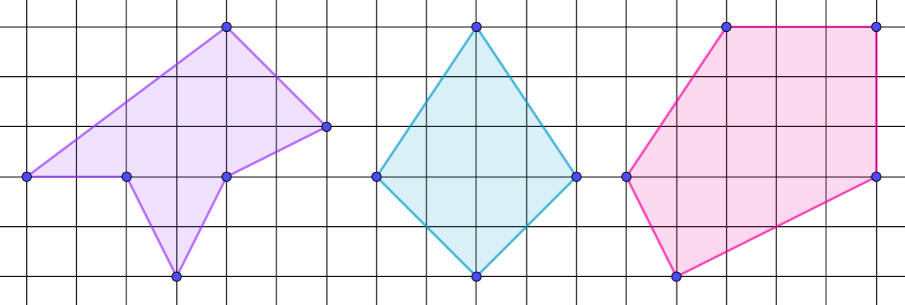
\includegraphics[width= 1\linewidth]{3}
		\caption{\small\textit{\color{toancuabi}Hình $3$. Đa giác đơn.}}
		\vspace*{-5pt}
	\end{figure}
	\begin{figure}[H]
		\vspace*{5pt}
		\centering
		\captionsetup{labelformat= empty, justification=centering}
		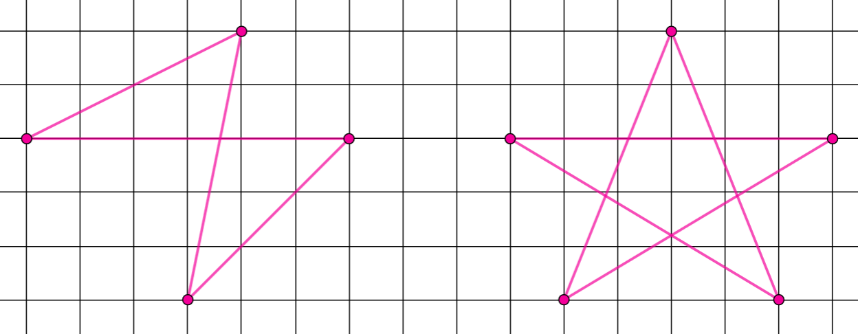
\includegraphics[width= 1\linewidth]{4}
		\caption{\small\textit{\color{toancuabi}Hình $4$. Đa giác không đơn.}}
		\vspace*{-10pt}
	\end{figure}
	Việc áp dụng định lý cho các đa giác không đơn có thể dẫn đến kết quả không chính xác. Các em ghi nhớ điều này khi dùng định lý Pick để tính diện tích nhé.
	\begin{figure}[H]
		\vspace*{-5pt}
		\centering
		\captionsetup{labelformat= empty, justification=centering}
		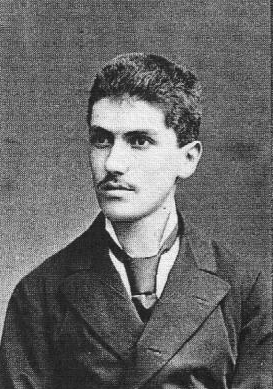
\includegraphics[width= 0.55\linewidth]{5}
		\caption{\small\textit{\color{toancuabi}Hình $5$. Georg Alexander Pick.}}
		\vspace*{-10pt}
	\end{figure}
	Định lý Pick được phát biểu đầy đủ như sau.
	\vskip 0.1cm
	$\pmb{2.}$ \textbf{\color{toancuabi}Tính diện tích theo định lý Pick}
	\vskip 0.1cm
	Trong mục này, chúng ta tính lại diện tích của một số hình trong Phần $1$ theo công thức có được từ định lý Pick và so sánh với nhau nhé.
	Đầu tiên là ``chú mèo" đáng yêu trong Ví dụ $4$ của Phần $1$.
	\vskip 0.1cm
	\textbf{\color{toancuabi}Ví dụ} $1$. Tính diện tích của hình được tô đậm dưới đây.
	\begin{figure}[H]
		\vspace*{-5pt}
		\centering
		\captionsetup{labelformat= empty, justification=centering}
		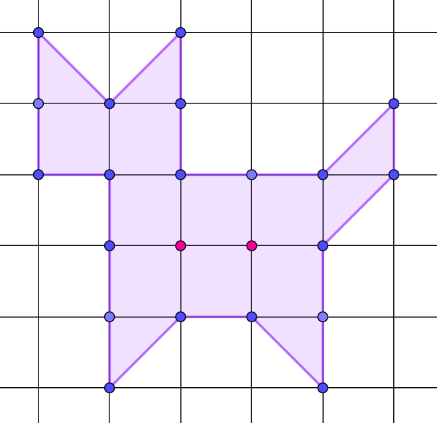
\includegraphics[width= 0.45\linewidth]{6}
		\caption{\small\textit{\color{toancuabi}Hình $6$.}}
		\vspace*{-10pt}
	\end{figure}
	\textit{Lời giải.} Ta dễ dàng thấy ngay $T = 2$ điểm trong ``chú mèo" và $B = 20$ điểm nằm trên các cạnh biên. Từ đó, diện tích của ``chú mèo" là:
	\begin{align*}
		T + \frac{B}{2} - 1 = 2 + \frac{20}{2} - 1 = 11 \text{ (đơn vị diện tích)}.
	\end{align*}
	Kết quả này cũng giống với con số mà ta đã tính được trong Phần $1$, nhưng có phần nhanh chóng hơn các em nhỉ.
	\vskip 0.1cm
	Chúng ta thử tiếp với hình trong Ví dụ $6$ trong Phần $1$.
	\vskip 0.1cm
	\textbf{\color{toancuabi}Ví dụ} $\pmb{2.}$ Tính diện tích của đa giác được tô đậm trong hình sau.
	\begin{figure}[H]
		\vspace*{-5pt}
		\centering
		\captionsetup{labelformat= empty, justification=centering}
		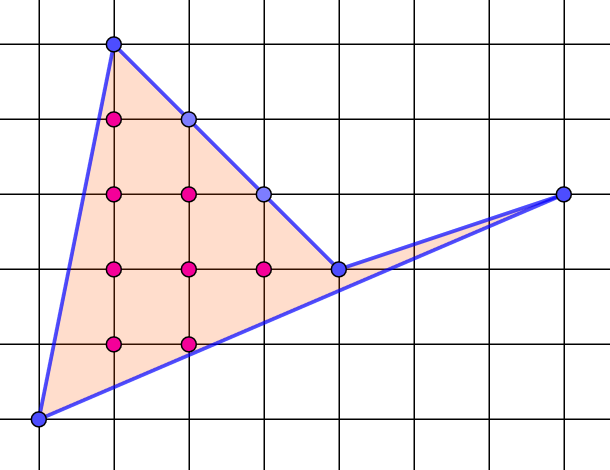
\includegraphics[width= 0.55\linewidth]{7}
		\caption{\small\textit{\color{toancuabi}Hình $7$.}}
		\vspace*{-10pt}
	\end{figure}
	\textit{Lời giải.}	Đa giác trong Hình $7$ có $T = 8$ điểm trong và $B = 6$ điểm nằm trên các canh. Do đó, Định lý Pick cho ta diện tích của đa giác này là:
	\begin{align*}
		T + \frac{B}{2} - 1 = 10 \text{ (đơn vị diện tích).}
	\end{align*}
	Kết quả này tất nhiên là trùng với con số tính ra theo cách giới thiệu ở Phần $1$ rồi, nhưng thay vì phải tính khá nhiều diện tích tam giác thông qua phương pháp lấy phần bù, chúng ta chỉ cần đếm số điểm nằm trên lưới. Định lý Pick thật là lợi hại phải không!
	\vskip 0.1cm
	Bài tập dưới đây để các em luyện tập thêm công thức Pick. Các em có thể tính diện tích theo cách trong Phần $1$ để kiểm tra lại nhé.
	\vskip 0.1cm
	\textbf{\color{toancuabi}Bài tập} $\pmb{1.}$ Tính diện tích của hình tô đậm sau đây.
	\begin{figure}[H]
		\vspace*{-5pt}
		\centering
		\captionsetup{labelformat= empty, justification=centering}
		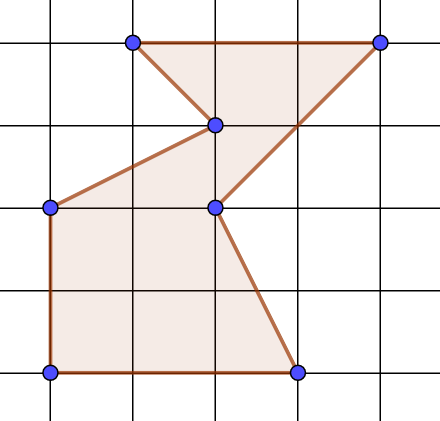
\includegraphics[width= 0.35\linewidth]{8}
		\caption{\small\textit{\color{toancuabi}Hình $8$.}}
		\vspace*{-5pt}
	\end{figure}
	$\pmb{3.}$ \textbf{\color{toancuabi}Làm thế nào để chứng minh định lý Pick?}
	\vskip 0.1cm
	Định lý Pick có thể chứng minh bằng nhiều cách khác nhau, trong khuôn khổ bài viết này, chúng ta chỉ mô tả cách tìm ra công thức của Pick cho hai hình cơ bản, đơn giản nhất -- hình chữ nhật và tam giác vuông có cạnh nằm trên lưới.
	\vskip 0.1cm 
	Nếu bạn nào quan tâm đến việc chứng minh đầy đủ định lý này thì có thể tham khảo các bước làm sau.
	\vskip 0.1cm
	-- Để chứng minh công thức Pick cho một đa giác nào đó ta chia đa giác thành hai phần bằng một đường chéo và quy về việc chứng công thức Pick cho mỗi đa giác thành phần. Ta thấy, đường chéo này trở thành cạnh của hai đa giác thành phần do đó các điểm nguyên trên đường chéo lúc trước được tính $1$ đơn vị, khi trở thành điểm biên thì tính $\dfrac{1}{2}$ đơn vị nhưng tính hai lần, vậy là hòa! Còn lại là hai điểm mút của đường chéo, chúng được tính hai lần do là đỉnh của hai đa giác con, vậy là dôi ra $1$ đơn vị. Nhưng trong công thức Pick sau khi tính các điểm biên và điểm trong ta bớt đi $1$ đơn vị. Đối với hai đa giác thành phần, ta bớt đi cả thảy $2$ đơn vị, vậy cũng hòa! 
	\begin{figure}[H]
		\vspace*{-5pt}
		\centering
		\captionsetup{labelformat= empty, justification=centering}
		
\includegraphics[width= 0.45\linewidth]{9}
		\caption{\small\textit{\color{toancuabi}Hình $9$.}}
		\vspace*{-10pt}
	\end{figure}
	-- Sau khi thực hiện nhiều lần chia đa giác thành các đa giác con, cuối cùng ta quy việc chứng minh định lý Pick cho tam giác. Ta lại tiếp tục chia tam giác đó thành các tam giác con nếu có một điểm nguyên ở trong hoặc trên biên tam giác. 
	\begin{figure}[H]
		\vspace*{5pt}
		\centering
		\captionsetup{labelformat= empty, justification=centering}
		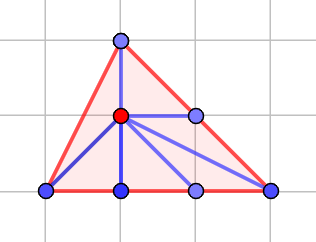
\includegraphics[width= 0.4\linewidth]{10}
		\caption{\small\textit{\color{toancuabi}Hình $10$.}}
		\vspace*{-10pt}
	\end{figure}
	-- Đối với tam giác không chứa điểm nguyên ở trong hoặc trên biên, định lý Pick khẳng định nó có diện tích bằng
	\begin{align*}
		\dfrac{3}{2}-1=\dfrac{1}{2} \text{ (đơn vị diện tích).}
	\end{align*}
	Dưới đây chúng ta sẽ xem một vài ví dụ kiểm chứng điều này. Hy vọng sau đó các bạn có thể tự đưa ra một chứng minh chặt chẽ của định lý Pick cho các tam giác đơn (nghĩa là tam giác không chứa điểm nguyên ở trong và trên biên, ngoại từ ba đỉnh).
	\begin{figure}[H]
		\vspace*{-5pt}
		\centering
		\captionsetup{labelformat= empty, justification=centering}
		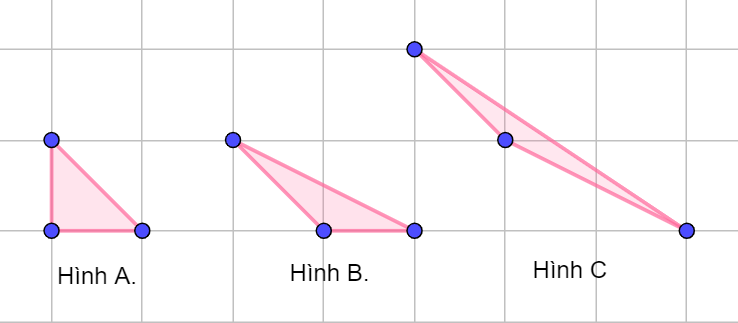
\includegraphics[width= 1\linewidth]{11}
		\caption{\small\textit{\color{toancuabi}Hình $11$.}}
		\vspace*{-10pt}
	\end{figure}
	Ba tam giác trong Hình $11$ đều là các tam giác đơn. Ba tam giác này có nhiều hình dáng khác nhau, nhưng ta đều thấy chúng có diện tích bằng $\dfrac{1}{2}$.
	Thật vậy, vận dụng những cách tính diện tích trong Phần $1$, ta có thể thấy ngay
	\begin{figure}[H]
		\vspace*{-5pt}
		\centering
		\captionsetup{labelformat= empty, justification=centering}
		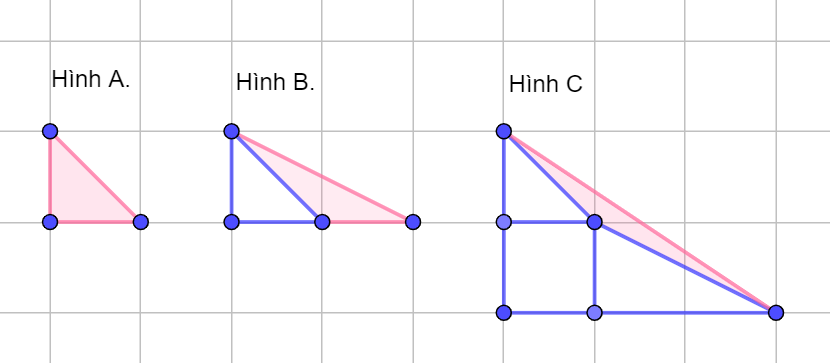
\includegraphics[width= 1\linewidth]{12}
		\caption{\small\textit{\color{toancuabi}Hình $12$.}}
		\vspace*{-10pt}
	\end{figure}
	-- Diện tích tam giác trong Hình $A$ là $\dfrac{1}{2}$;
	\vskip 0.1cm
	Diện tích của tam giác trong Hình $B$ là: 
	\begin{align*}
		\dfrac{1}{2}\times 1\times 2 - \dfrac{1}{2} = \dfrac{1}{2};
	\end{align*}
	Diện tích của tam giác trong Hình $C$ là: 
	\begin{align*}
		\dfrac{1}{2}\times2\times3 - \dfrac{1}{2} - 1 - \dfrac{1}{2}\times1\times2 = \dfrac{1}{2}.
	\end{align*}
	Bài viết về Tính diện tích trên lưới ô vuông đã giới thiệu đến các em cách tính diện tích của những hình trên lưới. Đầu tiên là hai phương pháp rất phổ biến: phương pháp chia hình cần tính thành những hình cơ bản đã biết diện tích và phương pháp tính theo phần bù. Tiếp theo đó bài viết giới thiệu với các em một công thức tính diện tích vô cùng đẹp đẽ qua Định lý Pick. Việc áp dụng định lý Pick giúp tính diện tích trở nên đơn giản hơn nhiều vì ta chỉ cần đếm số điểm nguyên ở trong và trên cạnh của hình cần tính. Chủ đề tính diện tích trên lưới ô vuông vẫn còn nhiều điều hấp dẫn, các bạn nhỏ nếu tìm được những bài toán hay thì hãy chia sẻ cùng Pi và các thầy cô trong câu lạc bộ UMC nhé.
\end{multicols}
\vspace*{-10pt}
{\color{toancuabi}\rule{1\linewidth}{0.1pt}}
\blfootnote{\color{toancuabi}$^1$THPT Chuyên Hưng Yên.}
\begingroup
\AddToShipoutPicture*{\put(126,452){
\includegraphics[scale=1]{../tieude10.pdf}}}
\centering
\endgroup
\vspace*{66pt}
\begin{multicols}{2}
	Các quốc gia trên thế giới có nhiều hình thức tổ chức đón năm mới khác nhau, trong đó phải kể đến việc phát hành tem bưu chính. Tem của các nước phương Tây gắn liền với dịp lễ Giáng sinh và ngày đầu năm mới. Phương Đông đón Tết theo lịch mặt trăng vì thế tem Tết các nước châu Á mang nhiều ý nghĩa văn hóa phương Đông. Đối với người xa Tổ quốc, mỗi khi nhận được lá thư hoặc bưu thiếp dán tem Tết lại gợi nhớ quê hương, cội nguồn, nhớ về ngày Tết cổ truyền của dân tộc mình và con tem cũng là hàm ý như lời chúc mừng năm mới từ người gửi đến người nhận. Lời chúc qua thư và bưu thiếp có tem Tết mang nét độc đáo riêng mà lời chúc qua hệ thống liên lạc khác không dễ thay thế. Tem như một lời nhắn gửi Tết là thời khắc thiêng liêng để vạn vật được hồi sinh, để những người con xa quê hương có cơ hội đoàn tụ bên gia đình, cùng nhau đón thời khắc giao thừa với mong ước những điều may mắn, hạnh phúc, bình an, tài lộc sẽ đến trong năm mới. Tem Tết được phát hành hàng năm như lời chúc về một năm mới trăm điều an khang, vạn điều may mắn, mã đáo thành công, lộc đến nhà nhà.
	\vskip 0.1cm 
	Một trong những chủ đề không thể thiếu trên tem Tết ở các nước châu Á là hình tượng $12$ con giáp. Tính theo cung hoàng đạo, năm mới gắn với con vật nào thì con vật đó được các họa sĩ thể hiện trên tem để tôn vinh vẻ đẹp và ý nghĩa của nó như một linh vật trong năm. Tháng $8$ năm $1998$ tại hội thảo quốc tế về tem thư tổ chức tại Israel, tem $12$ con giáp được bầu chọn là đề tài đứng thứ $2$ trong bảng xếp hạng $10$ đề tài tem thư lưu hành phổ biến nhất trên thế giới. Điều này cho thấy văn hóa mười hai con giáp của phương Đông đã có sức hấp dẫn lôi cuốn những khu vực khác trên thế giới.
	\vskip 0.1cm 
	Hiện nay, có khoảng $80$ nước và các vùng lãnh thổ ở châu Á, châu Phi, châu Mỹ phát hành những bộ tem về động vật liên quan đến $12$ con giáp. Nước đầu tiên phát hành tem về các con giáp là Nhật Bản, tiếp đến là Hàn Quốc và Trung Quốc. Tết cổ truyền là một trong những dịp lễ trọng đại nhất trong năm ở Việt Nam, đóng vai trò rất quan trọng trong đời sống tinh thần của người Việt. Tem phát hành dịp Tết ở Việt Nam, cùng chung dòng chảy với văn hóa phương Đông nhưng nó được tiếp nhận, chắt lọc, sáng tạo biến cách trên nền tảng bản sắc dân tộc Việt. Tem Tết đầu tiên về con giáp ở Việt Nam được phát hành vào ngày $16$ tháng $1$ năm $1962$ với mẫu tem Tranh Tết Đông Hồ gồm hai mẫu \textit{Lợn lái, lợn con} và \textit{Gà mái, gà con} đều dựa theo tranh khắc gỗ dân gian Đông Hồ, một loại hình truyền thống dân tộc. 
	\begin{figure}[H]
		\vspace*{-5pt}
		\centering
		\captionsetup{labelformat= empty, justification=centering}
		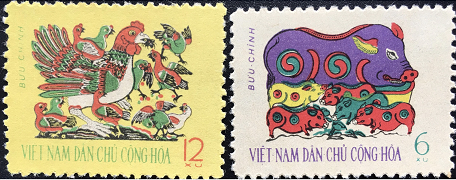
\includegraphics[width= 1\linewidth]{tem1}
		\vspace*{-15pt}
	\end{figure}
	Chuẩn bị bước sang năm mới Quý Mão ngày $1.12.2022$  Bộ Thông tin và Truyền thông phát hành bộ tem bưu chính “Tết Quý Mão” gồm $2$ mẫu tem và $1$ blốc do họa sĩ Nguyễn Quang Vinh thiết kế. Con Mèo trên tem được thể hiện theo phong cách hiện đại, đường nét dứt khoát, mạnh mẽ nhưng cũng thể hiện sự mềm mại, uyển chuyển. 
	\begin{figure}[H]
		\vspace*{-5pt}
		\centering
		\captionsetup{labelformat= empty, justification=centering}
		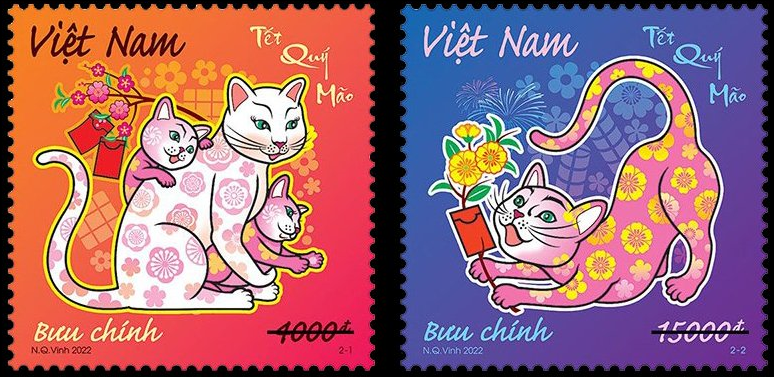
\includegraphics[width= 1\linewidth]{tem2}
		\vspace*{-15pt}
	\end{figure}
	Ở trung tâm mẫu tem thứ nhất là hình ảnh mèo mẹ và hai chú mèo con đang quấn quýt, vui đùa. Mèo mẹ ôm và cõng mèo con trên lưng cũng như biết bao người mẹ trên cuộc đời: vừa bao dung ôm trọn con vào lòng, bảo vệ con trước giông tố, sóng gió; vừa sẵn sàng "cõng" con, cùng con vượt bao khó khăn, vất vả trong cuộc sống. Hình ảnh mèo cha ở mẫu tem thứ hai được khắc họa trên nền tem màu xanh sắc lạnh, tạo liên tưởng đến hình ảnh người cha đầy mạnh mẽ, có phần "đơn độc", một mình gánh vác cả "thế giới" trên lưng để bảo vệ sự bình yên cho gia đình nhỏ của mình. Các chú mèo trong hai mẫu tem được sắp xếp đối xứng, hướng vào nhau như mong ước về đoàn viên, sum vầy ngày Tết được thể hiện trên mẫu blốc tem. Khung cảnh ấm áp của gia đình mèo gợi cho người xem một nỗi nhớ nhung, như thúc giục mọi người hãy nhanh nhanh sắp xếp công việc, bắt chuyến tàu Tết để về với gia đình, bởi ở đó mới thực sự là khung trời bình yên, để ta yên tâm bỏ lại những bộn bề, lo âu của cuộc sống và tận hưởng những phút giây hạnh phúc bên người thân yêu.
	\begin{figure}[H]
		\vspace*{-5pt}
		\centering
		\captionsetup{labelformat= empty, justification=centering}
		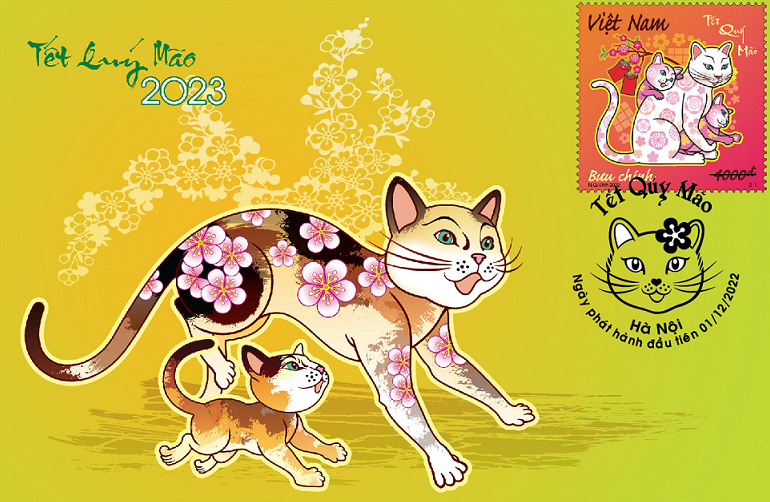
\includegraphics[height=0.382\linewidth]{tem3}
		
\includegraphics[height=0.382\linewidth]{tem4}
		\vspace*{-10pt}
	\end{figure}
	Các hình ảnh quen thuộc của ngày Tết như hoa đào, hoa mai, bánh chưng, bánh dày và bao lì xì đỏ cũng được thể hiện trên bloc. Đàn chim én tung bay được khắc họa trên nền blốc tem báo hiệu một năm mới rộn ràng, đầy hứa hẹn sắp đến. 
	\vskip 0.1cm
	Với các bạn đọc nhỏ tuổi của Pi, chúng ta hãy cùng thử sức với một số bài toán về tem sau đây nhé.
	\vskip 0.1cm
	\textbf{\color{toancuabi}Bài toán} $\pmb{1.}$ Có bao nhiêu cách dán $3$ tem thư khác nhau lên $3$ bì thư khác nhau?
	\vskip 0.1cm
	\textit{Lời giải.} Trước hết sắp xếp ba con tem theo thứ tự nào đó và lần lượt dán chúng:
	\vskip 0.1cm
	$\circ$	Chọn một bì thư để dán con tem thứ nhất: ta có $3$ cách làm như vậy.
	\vskip 0.1cm
	$\circ$	Chọn một bì thư trong số hai bì còn lại để dán tem thư thứ hai: ta có $2$ cách làm như vậy.
	\vskip 0.1cm
	$\circ$	Dán tem thư cuối cùng lên bì thư còn lại: ta  có $1$ cách làm.
	\vskip 0.1cm
	Do đó số cách dán ba tem thư khác nhau lên ba bì thư khác nhau là
%	\setlength{\abovedisplayskip}{7pt}
%	\setlength{\belowdisplayskip}{7pt}
	\begin{align*}
		3 \times 2 \times 1= 6 \text{ (cách).}
	\end{align*}
	\textbf{\color{toancuabi}Bài toán} $\pmb{2.}$ Minh thích chơi tem, bạn ấy đã sưu tầm được $450$ tem, được chia ra thành cách loại như sau: có $70$ tem phát hành ở các nước châu Mỹ, $210$ tem phát hành ở các nước châu Á và số tem còn lại được phát hành ở các nước châu Phi. Minh muốn chia đều mỗi loại tem phát hành ở các châu lục đó để ép vào các album tem. Hỏi có bao nhiêu cách chia với số album nhiều hơn $1$ (hai cách chia là như nhau nếu số tem mỗi loại trong một album là bằng nhau)? Số album cần có để mỗi album có số tem ít nhất là bao nhiêu? Tính số tem mỗi loại trong các album trong mỗi cách chia đó.
	\vskip 0.1cm
	\textit{Lời giải.}
	Số tem được phát hành ở các nước châu Phi là:
	\begin{align*}
		450 - 70 - 210 =170  \text{ (tem).}
	\end{align*}
	Gọi số album là $x$  ($x \in \mathbb{N^*}$).
	\vskip 0.1cm
	Ta có:
	\begin{align*}
		&70\,\,\vdots\,\, x, 210\,\,\vdots\,\, x; 170 \,\,\vdots\,\, x\\
		\Rightarrow & x \in  \text{ƯC}(70,210,170), 
	\end{align*}
	mà
	\begin{align*}
		&\text{ƯCLN}(70,210,170)=10 \\
		\Rightarrow &x \in \text{Ư}(10)=\{1,2,5,10\}
	\end{align*}
	Do đó số cách chia tem với số album nhiều hơn $1$ sẽ là $3$ cách: cách $1$ dùng $2$ album, cách $2$ dùng $5$ album và cách thứ ba dùng $10$ album.  
	Để số tem trong mỗi album là ít nhất thì Minh cần dùng số album là lớn nhất có thể, có nghĩa là Minh cần $10$ album.
	\vskip 0.1cm
	Nếu chia thành $2$ album thì số tem trong mỗi album là  $450 : 2 = 225$
	\vskip 0.1cm  
	Nếu chia thành $5$ album thì số tem trong mỗi album là $450:5=90$ 
	\vskip 0.1cm
	Nếu chia thành $10$ album thì số tem trong mỗi album là $450:10 = 45$
	\vskip 0.1cm 
	\textbf{\color{toancuabi}Bài toán} $\pmb{3.}$ Anh Hưng là nhà sưu tập tem và có nhiều bạn cùng sở thích. Dịp Tết Nhâm Dần, Bộ Thông tin và Truyền thông phát hành bộ tem bưu chính gồm $2$ mẫu tem và $1$ blốc với giá lần lượt $4$ nghìn đồng, $15$ nghìn đồng và $38$ nghìn đồng. Anh Hưng đến Bưu điện thành phố mua để tặng bạn bè những sản phẩm mới đó với $600$ nghìn đồng. Anh muốn số tem loại $4$ nghìn đồng gấp $10$ lần số blốc và dung hết số tiền để mua tem $15$ nghìn đồng”. Theo bạn thì Hưng nhận được bao nhiêu chiếc cho mỗi loại tem và blốc? 
	\vskip 0.1cm
	\textit{Lời giải.}
	Gọi $x$ là số blốc, $y$ là số tem loại $15$ nghìn đồng. Khi đó số tem loại $4$ nghìn đồng là $10x$  ($x, y \in \mathbb{N^*}$)
	\vskip 0.1cm
	Khi đó  $10x \cdot 4 +15\cdot y +38\cdot y =600$. Từ đó 
	\begin{align*}
		78x + 15y = 600. \tag{$1$}
	\end{align*}
	Ta có  $78x = 600 - 15y = 15(40-y)$. Suy ra $78x < 600$  và $78x$ chia hết cho $5$. Từ đó, ta có  $x < 8$ và do đó $x = 5$. Thay vào phương trình ($1$) ta thu được $78 \cdot 5 + 15y = 600$, dẫn đến $15y = 210$ và vì thế $y = 14$.
	\vskip 0.1cm
	Như vậy, anh Hưng nhận được $50$ tem loại $4$ nghìn đồng, $14$ tem loại $15$ nghìn đồng và $5$ blốc giá $38$ nghìn đồng.
	\vskip 0.1cm
	Cuối cùng mời các bạn đọc nhỏ tuổi thử sức với hai bài toán sau.
	\vskip 0.1cm
	\textbf{\color{toancuabi}Bài} $\pmb{1.}$ Hai bạn Minh và Hải chơi tem thư. Nếu Minh cho Hải một số tem bằng số con tem mà Hải sưu tầm được, rồi Hải lại cho Minh một số tem bằng số tem còn lại của Minh thì kết quả là Minh sẽ có số tem nhiều hơn số mà Minh đã sưu tầm được là $30$ con tem và khi đó Hải có số tem bằng một phần ba lần số tem mà Hải sưu tầm được. Hỏi số tem mà mỗi bạn đã sưu tầm được là bao nhiêu?
	\vskip 0.1cm
	\textbf{\color{toancuabi}Bài} $\pmb{2.}$ Có $3$ tem thư khác nhau và $6$ bì thư cũng khác nhau. Hỏi có bao nhiêu cách dán $3$ tem thư lên $3$ trong $6$ bì thư đó ?
\end{multicols}
\newpage
\begingroup
\AddToShipoutPicture*{\put(121,645){
\includegraphics[scale=1]{../tieude.pdf}}} 
\centering
\endgroup
\vspace*{60pt}
\begin{multicols}{2}
	Thám tử Xuân Phong và thanh tra Lê Kính nhân dịp đi điều tra ở vùng xa được mời tới thăm quan một thành phố kỳ lạ được mang tên Thành phố Thông minh. Thành phố chỉ có vẻn vẹn $200$ cư dân, họ ở trong những ngôi nhà cực kỳ hiện đại với nhiều tiện nghi tối tân và đặc biệt hơn, cư dân được chia ra thành $3$ loại người: $a)$ Người \textit{ngốc ngếch} luôn coi tất cả mọi người khác là ngốc ngếch còn mỗi mình là thông minh; $b)$ người \textit{thông minh khiêm tốn} biết chính xác về tất cả những người khác, còn coi bản thân là ngốc ngếch; $c)$ người \textit{thông minh tự tin} biết chính xác về tất cả những người khác và coi mình là thông minh. Theo thói quen nghề nghiệp, Xuân Phong liền mời tất cả công dân của thành phố tới tòa thị chính để mở một cuộc điều tra khảo sát ẩn danh về câu hỏi: trong tòa thị chính bây giờ có tất cả bao nhiêu công dân của thành phố là thông minh? Sau khi thu phiếu điều tra về, Xuân Phong không thể nào xác định được số lượng công dân thông minh của thành phố. Bỗng dưng vừa đúng lúc đó có một công dân trở về sau chuyến du lịch và chưa kịp tham gia trả lời khảo sát cùng với $199$ công dân đứng chật ních ở tòa thị chính. Anh ta nhanh chóng nhận phiếu điều tra, điền thông tin về các công dân trong phòng thị chính, kể cả về bản thân. Xuân Phong đọc câu trả lời của công dân đến muộn này và nói nhỏ cho Lê Kính “Giờ thì tôi cũng biết rõ về số các nhà thông minh trong thành phố này rồi”.
	\vskip 0.1cm
	Vậy theo em trong thành phố đặc biệt nọ có thể có bao nhiêu công dân thông minh?
	\begin{figure}[H]
		\centering
		\vspace*{-10pt}
		\captionsetup{labelformat= empty, justification=centering}
		\includegraphics[width=1\linewidth]{Pi1_2_XuanPhong}
		\vspace*{-5pt}
	\end{figure}	
	%	Tất cả các người \textit{ngốc ngếch} đều trả lời “Một”. Nếu trong tòa thị chính  có ít nhất là $3$ công dân thông minh, thì tất cả họ sẽ đưa ra một số không nhỏ hơn $2$, và Xuân Phong đã biết được ngay câu trả lời. Vì thế, số công dân thông minh chỉ có thể là $0$, $1$ hoặc $2$. Ta xét tất cả các trường hợp.
	%	\vskip 0.1cm
	%	Nếu không có công dân thông mình nào, thì tất cả sẽ trả lời là “Một”. Nếu chỉ có một công dân thông minh và hơn nữa lại tự tin, thì anh ta cũng trả lời “Một” và tình huống này không phân biệt được với tình huống trước. Nếu người thông minh duy nhất là khiêm tốn, thì anh ta sẽ trả lời “Không có ai”, và trường hợp này phân biệt được ngay.
	%	\vskip 0.1cm
	%	Nếu có hai công dân thông minh và lại khiêm tốn, thì họ cũng lại trả lời “Một”, và tình huống này không phân biệt được với tình huống thứ nhất. Còn nếu có hai công dân thông minh và cả hai lại tự tin, thì họ sẽ đều trả lời “Hai”, tình huống này phân biệt được rõ ngay. Còn nếu có một công dân thông minh tự tin và một công dân thông minh khiêm tốn, thì người thông minh tự tin cũng trả lời “Hai” và tình huống phân biệt được.
	%	\vskip 0.1cm
	%	Như vậy, chỉ có thể có $3$ trường hợp không phân biệt được rõ ràng khi khảo sát $199$ công dân: không có công dân thông minh nào, có một người thông minh tự tin, và có hai người thông minh khiêm tốn. Trong cả $3$ phương án này tất cả các phiếu điều tra đều ghi “Một”.
	%	\vskip 0.1cm
	%	Giờ ta sẽ xem, người tới muộn sẽ đưa ra những câu trả lời nào trong mỗi tình huống được nêu ở trên, phụ thuộc vào mức độ thông minh và khiêm tốn của anh ta.
	%	\vskip 0.1cm
	%	\begin{table}[H]
		%		\vspace*{-5pt}
		%		\centering
		%		\captionsetup{labelformat= empty, justification=centering}
		%		\begin{tabular}{|l|c|c|c|}
			%			\hline
			%			& $0$ người thông minh tự tin
			%			$0$ người thông minh khiêm tốn&	$1$ người thông minh tự tin
			%			$0$ người thông minh khiêm tốn&	$0$ người thông minh tự tin
			%			$2$ người thông minh khiêm tốn\\
			%			\hline
			%			Ngốc ngếch &	$1$&	$1$&	$1$\\
			%			\hline
			%			Tự tin	&$1$ &	$2$&	$3$\\
			%			\hline
			%			Khiêm tốn&	$0$&	$1$&	$2$\\
			%			\hline
			%		\end{tabular}
		%		\vspace*{-10pt}
		%	\end{table}
	%	Ta thấy rõ ràng là các câu trả lời “$1$” và “$2$” đều được gặp ở vài ô, có nghĩa là chúng không giúp gì được cho việc phân biệt các tình huống. Tuy nhiên các trả lời “$0$” và “$3$”
	%	lại gặp đúng một lần, và chúng cho phép đưa ra các kết luận duy nhất. Vì thế người tới muộn đã đưa ra một trong các câu trả lời đó. Trong trường hợp anh ta trả lời “$0$”
	%	thì trong thành phố có duy nhất $1$ công dân thông minh (là chính người tới muộn đó), còn trong trường hợp anh ta trả lời “$3$” thì đúng là trong thành phố có $3$ công dân thông minh ($2$ người khiêm tốn và $1$ người tự tin là anh tới muộn đó).
	%	\vskip 0.1cm
	%	Đáp số: $1$ hoặc $3$.
\end{multicols}
\newpage
\begingroup
\AddToShipoutPicture*{\put(112,672){
\includegraphics[scale=1]{../tieude11.pdf}}} 
\centering
\endgroup
\vspace*{35pt}

\begin{multicols}{2}
	$\pmb{1.}$ Một bác nông dân chở một xe ô tô quất cảnh ra chợ Tết để bán. Sau khi bán hết cây quất cuối cùng với giá $230$ nghìn đồng, bác tính nhẩm lại thấy mình đã bán số cây quất với giá trung bình là $245$ nghìn đồng/cây. Nhưng ngay lúc ấy người mua cây quất cuối quay trở lại và chỉ cho bác thấy cành quất bị rụng quá nhiều lá, nên ông ta chỉ đồng ý mua với giá $158$ nghìn đồng. Bác chấp thuận và bán cành quất đó. Khi nhẩm tính lại, bác nông dân thấy giá trung bình của xe quất bây giờ là $242$ nghìn đồng. Hỏi bác đã bán được bao nhiêu cây quất?
	\begin{figure}[H]
		\centering
		\vspace*{-10pt}
		\captionsetup{labelformat= empty, justification=centering}
		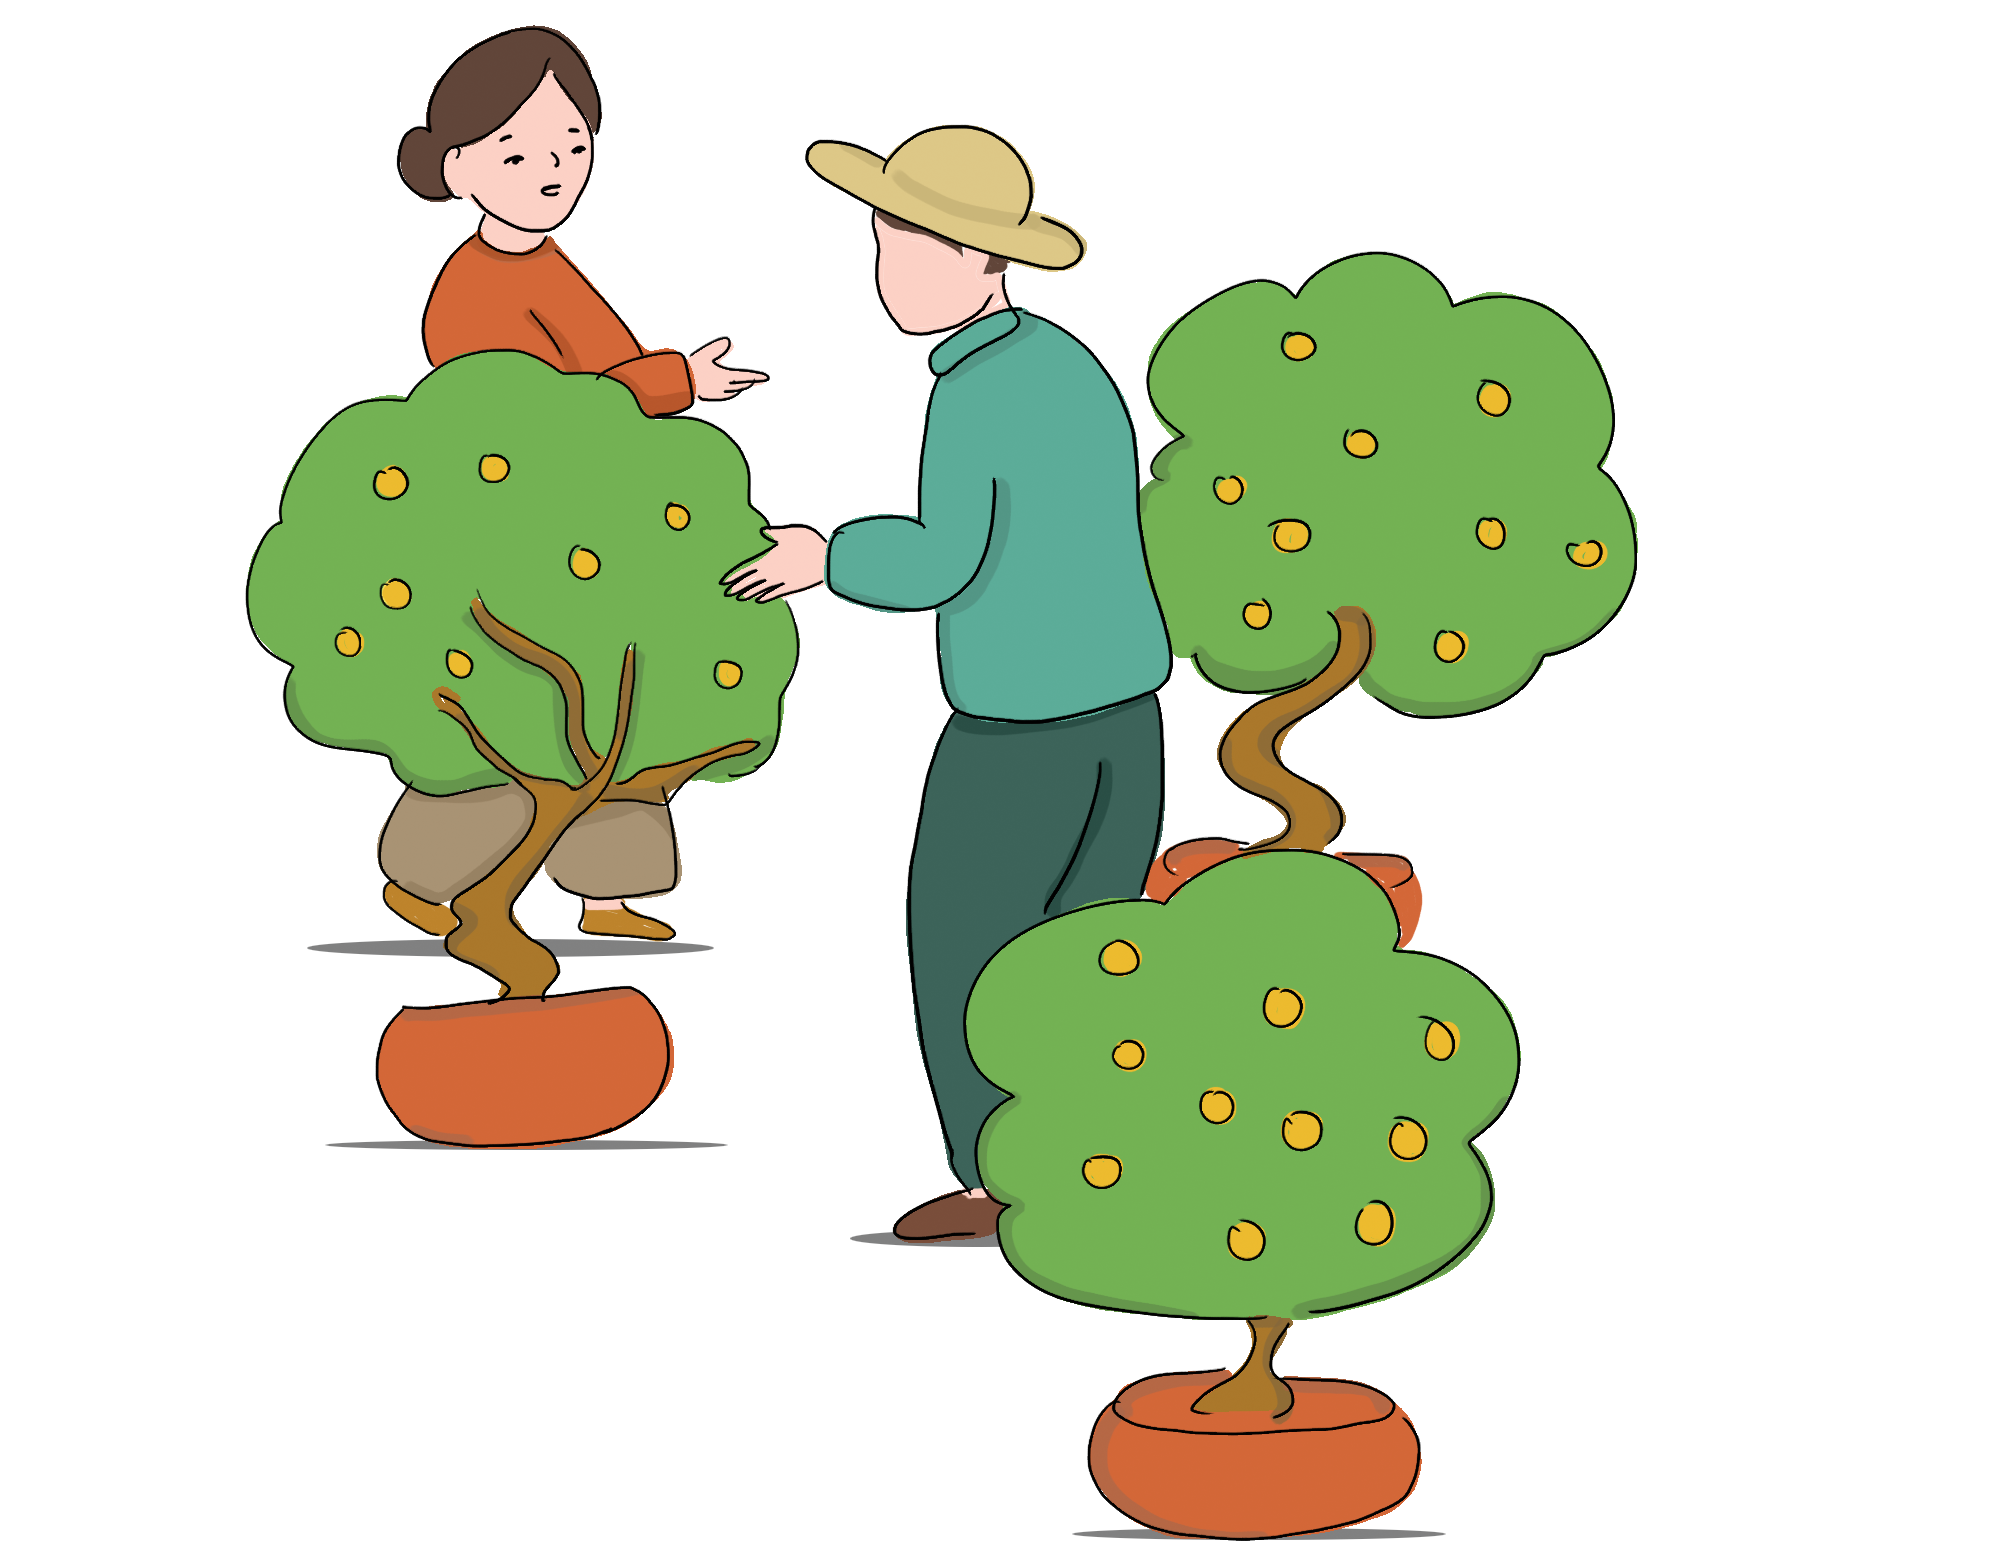
\includegraphics[width=0.8\linewidth]{Pi1_2_Bai1}
		\vspace*{-10pt}
	\end{figure}
	$\pmb{2.}$ Chuyện kể rằng có một người khi gặp nhà triết học và toán học Hy--lạp Pythagoras đã hỏi ông: “Bây giờ là mấy giờ?” Pythagoras đã trả lời “Cho đến hết ngày còn lại hai lần của hai phần năm khoảng thời gian đã trôi qua từ lúc bắt đầu ngày”. Nghe vậy, người đó chịu không thể nghĩ ra ngay được lúc họ gặp nhau là mấy giờ. Em có thể giúp trả lời lúc đó là mấy giờ được không?
	\begin{figure}[H]
		\centering
		\vspace*{-10pt}
		\captionsetup{labelformat= empty, justification=centering}
		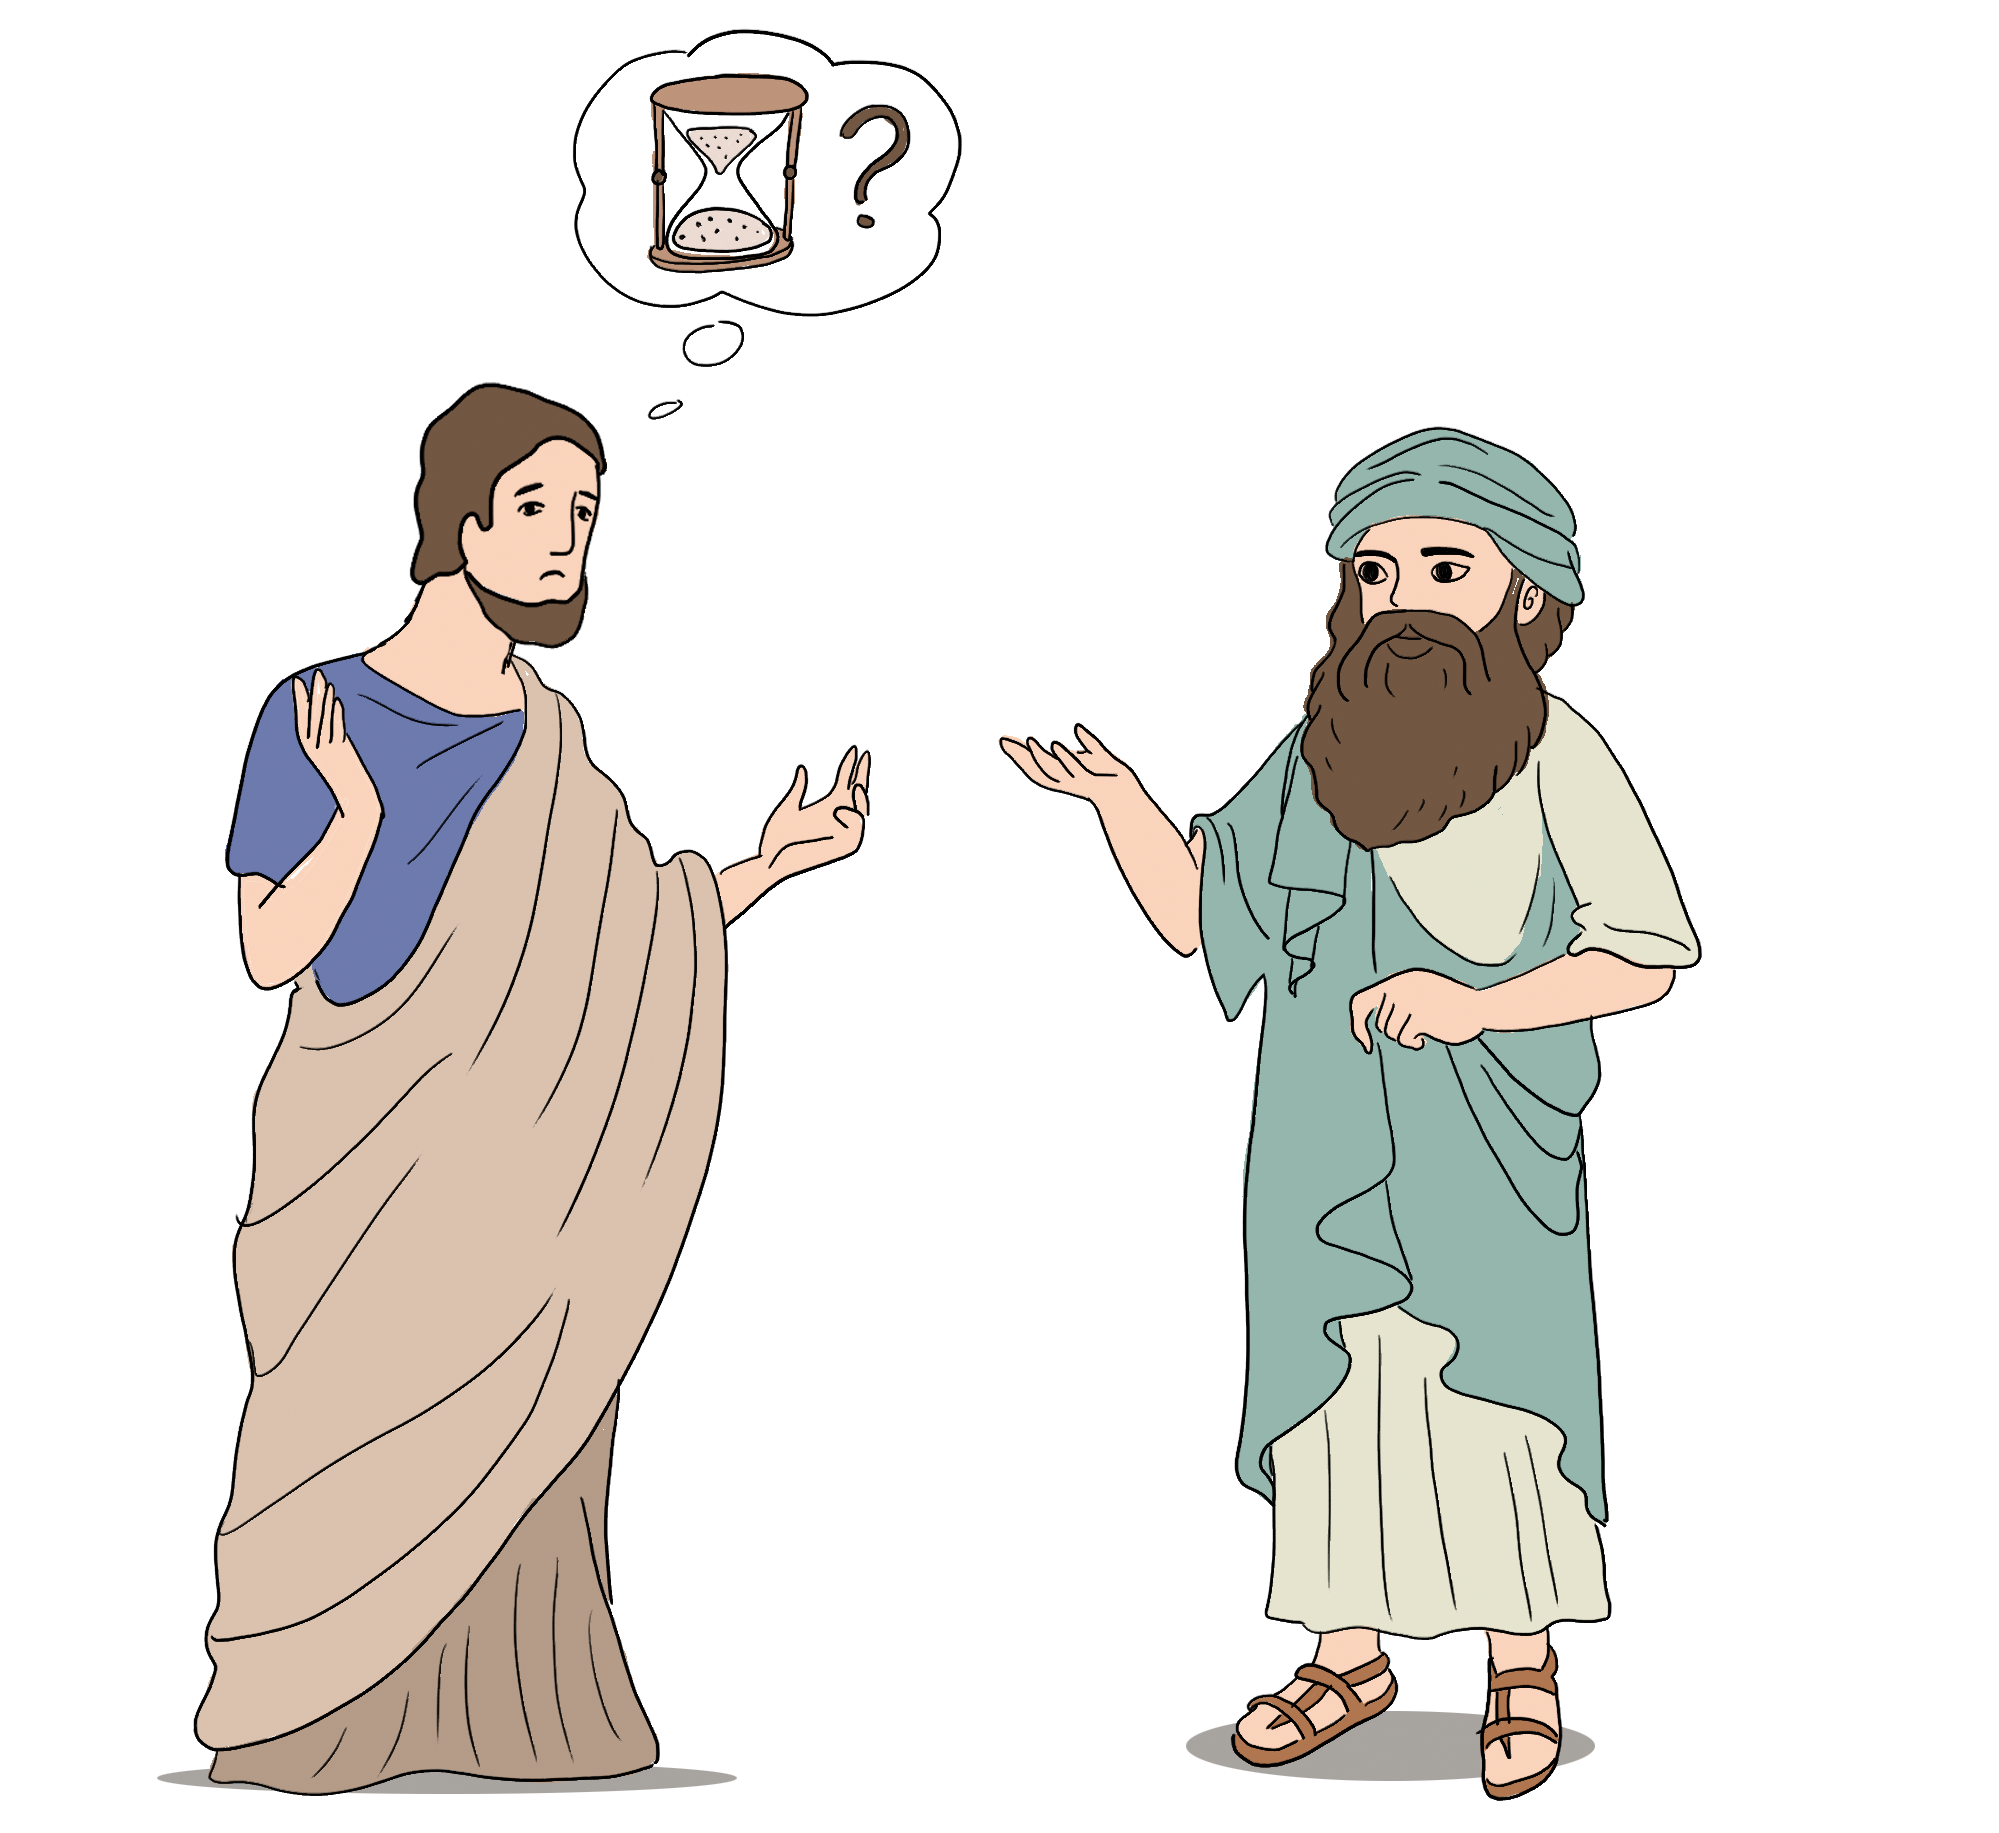
\includegraphics[width=0.7\linewidth]{Pi1_2_Bai2}
		\vspace*{-5pt}
	\end{figure}
	$\pmb{3.}$ Một tháng trước bà Hoa ra chợ mua một cân khoai tây, một cân thịt và một chục trứng. Chủ nhật vừa rồi, khoai tây tăng lên gấp ba, thịt gấp $4$ lần còn trứng đắt gấp $5$ lần, nên bà Hoa phải trả $600$ nghìn cho từng ấy món hàng như lần thứ nhất. Hôm nay thì khoai lại đắt gấp $6$ lần so với tháng trước, thịt đắt gấp $5$ lần còn trứng chỉ đắt gấp $4$ lần nên bà Hoa lại phải trả $660$ nghìn với cùng một lượng hàng. Hỏi bà Hoa đã trả bao nhiêu tiền cho lần mua thứ nhất?
	\begin{figure}[H]
		\centering
		\vspace*{-10pt}
		\captionsetup{labelformat= empty, justification=centering}
		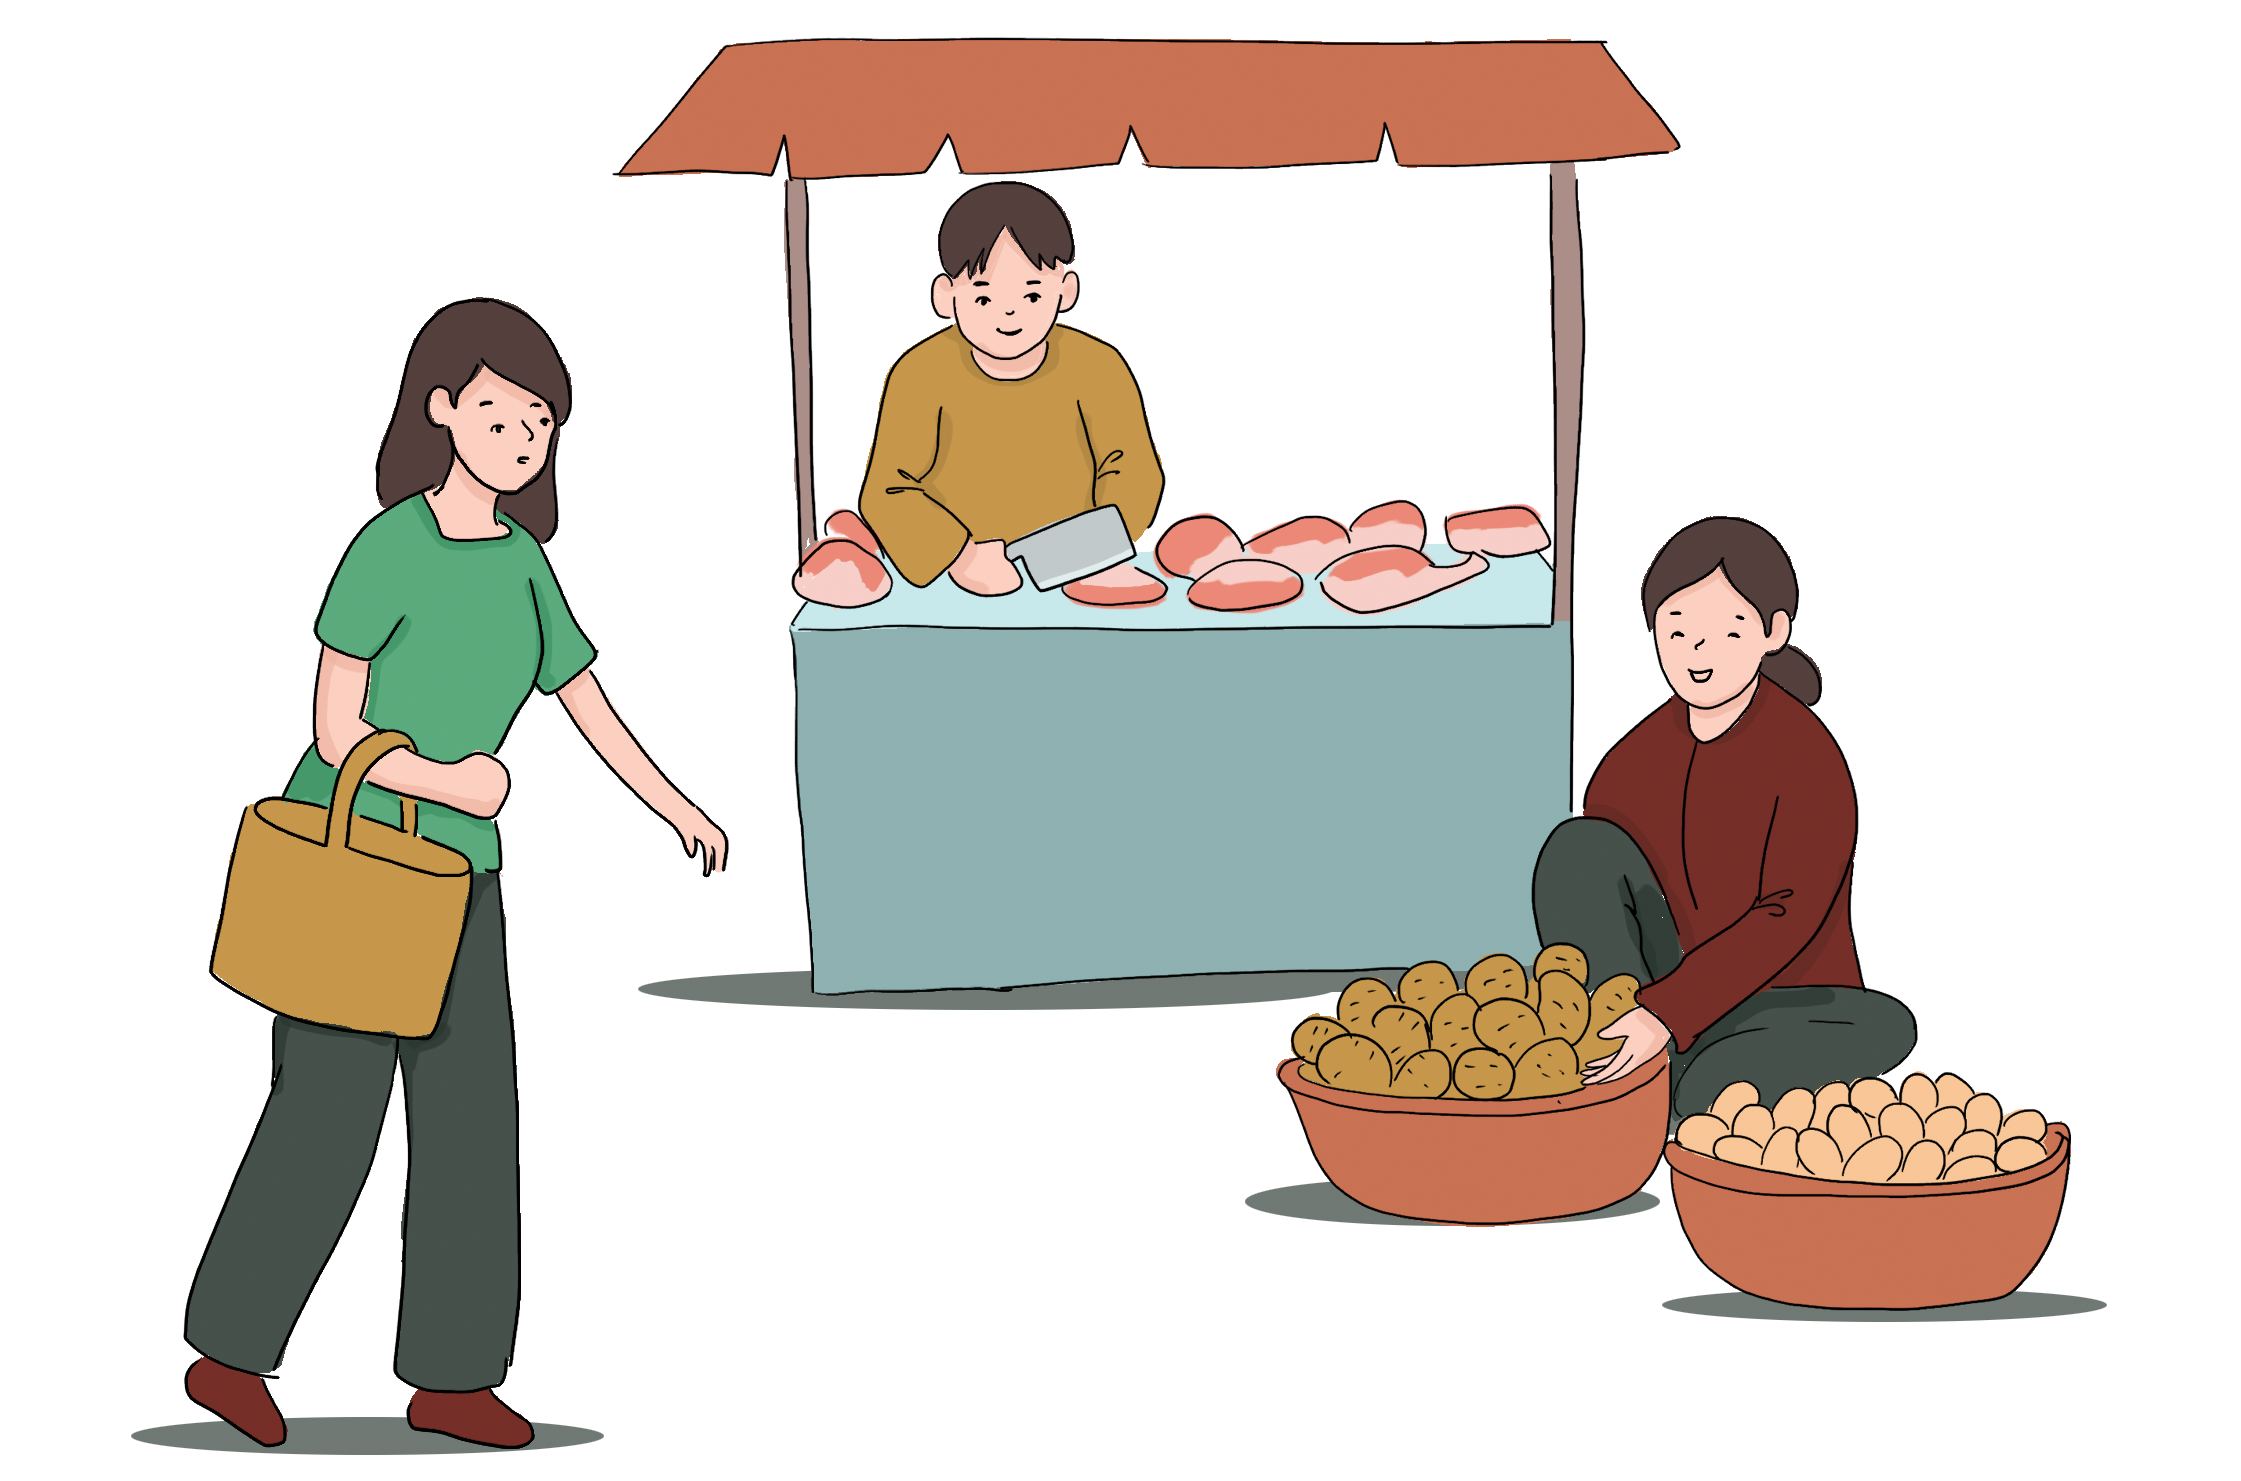
\includegraphics[width=0.9\linewidth]{Pi1_2_Bai3}
		\vspace*{-10pt}
	\end{figure}
	$\pmb{4.}$ Trong một buổi dạ hội nọ mỗi quý ông đã hân hạnh khiêu vũ với ba quý bà, còn mỗi quý bà cũng đã khiêu vũ với ba quý ông. Em hãy chỉ ra rằng số quý ông và số quý bà tham gia dạ hội là bằng nhau.
	\begin{figure}[H]
		\centering
		\vspace*{-5pt}
		\captionsetup{labelformat= empty, justification=centering}
		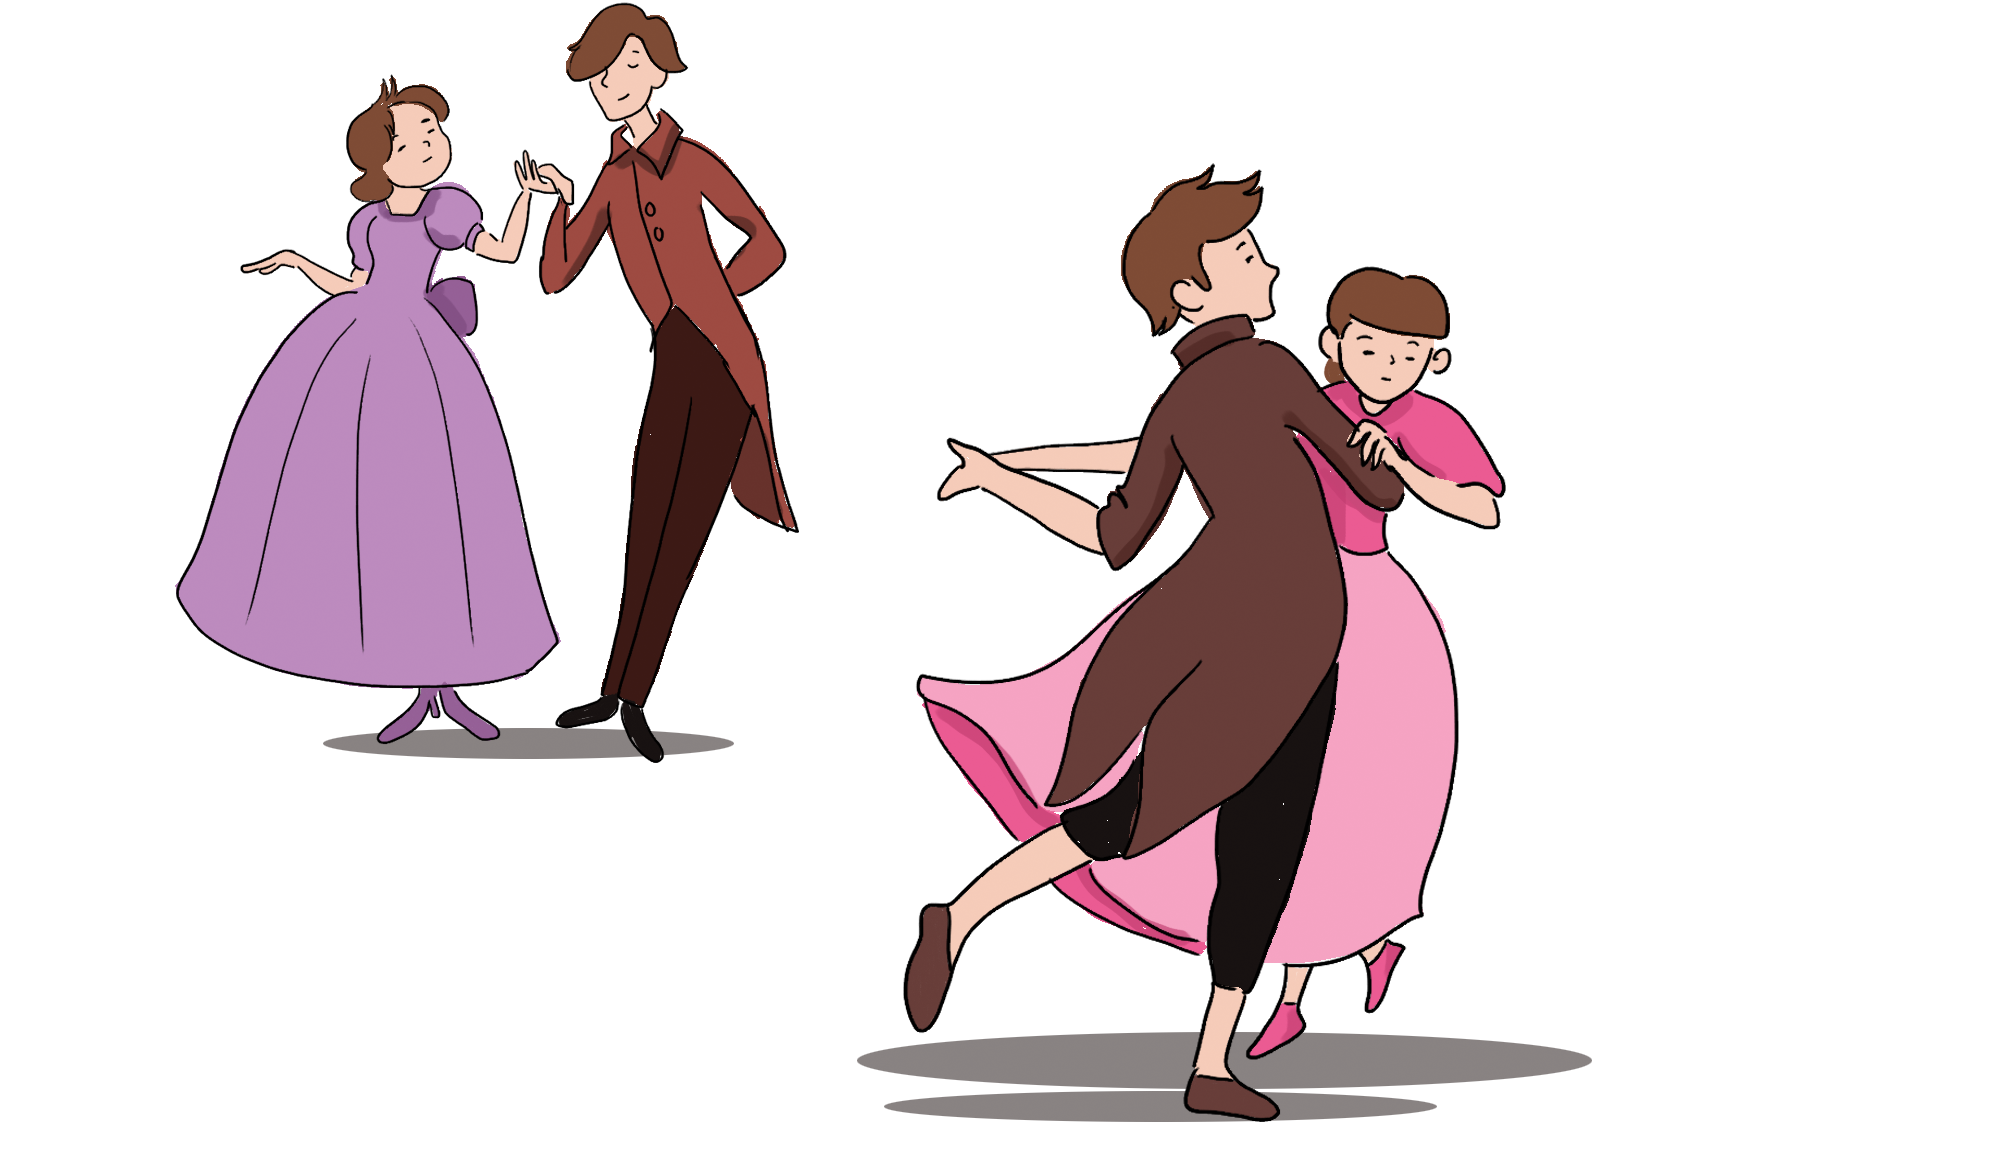
\includegraphics[width=1\linewidth]{Pi1_2_Bai4}
		\vspace*{-20pt}
	\end{figure}
	$\pmb{5.}$ 	Sau khi kết thúc một giải thi đấu cờ, ban tổ chức nhận thấy mỗi kỳ thủ tham gia đã có số trận thắng khi chơi bằng quân trắng bằng đúng số trận mà tất cả các kỳ thủ còn lại đã thắng khi chơi quân đen. Em hãy chỉ ra rằng tất cả các kỳ thủ tham gia thi đấu đã có số trận thắng là như nhau.
	\begin{figure}[H]
		\centering
		\vspace*{2pt}
		\captionsetup{labelformat= empty, justification=centering}
		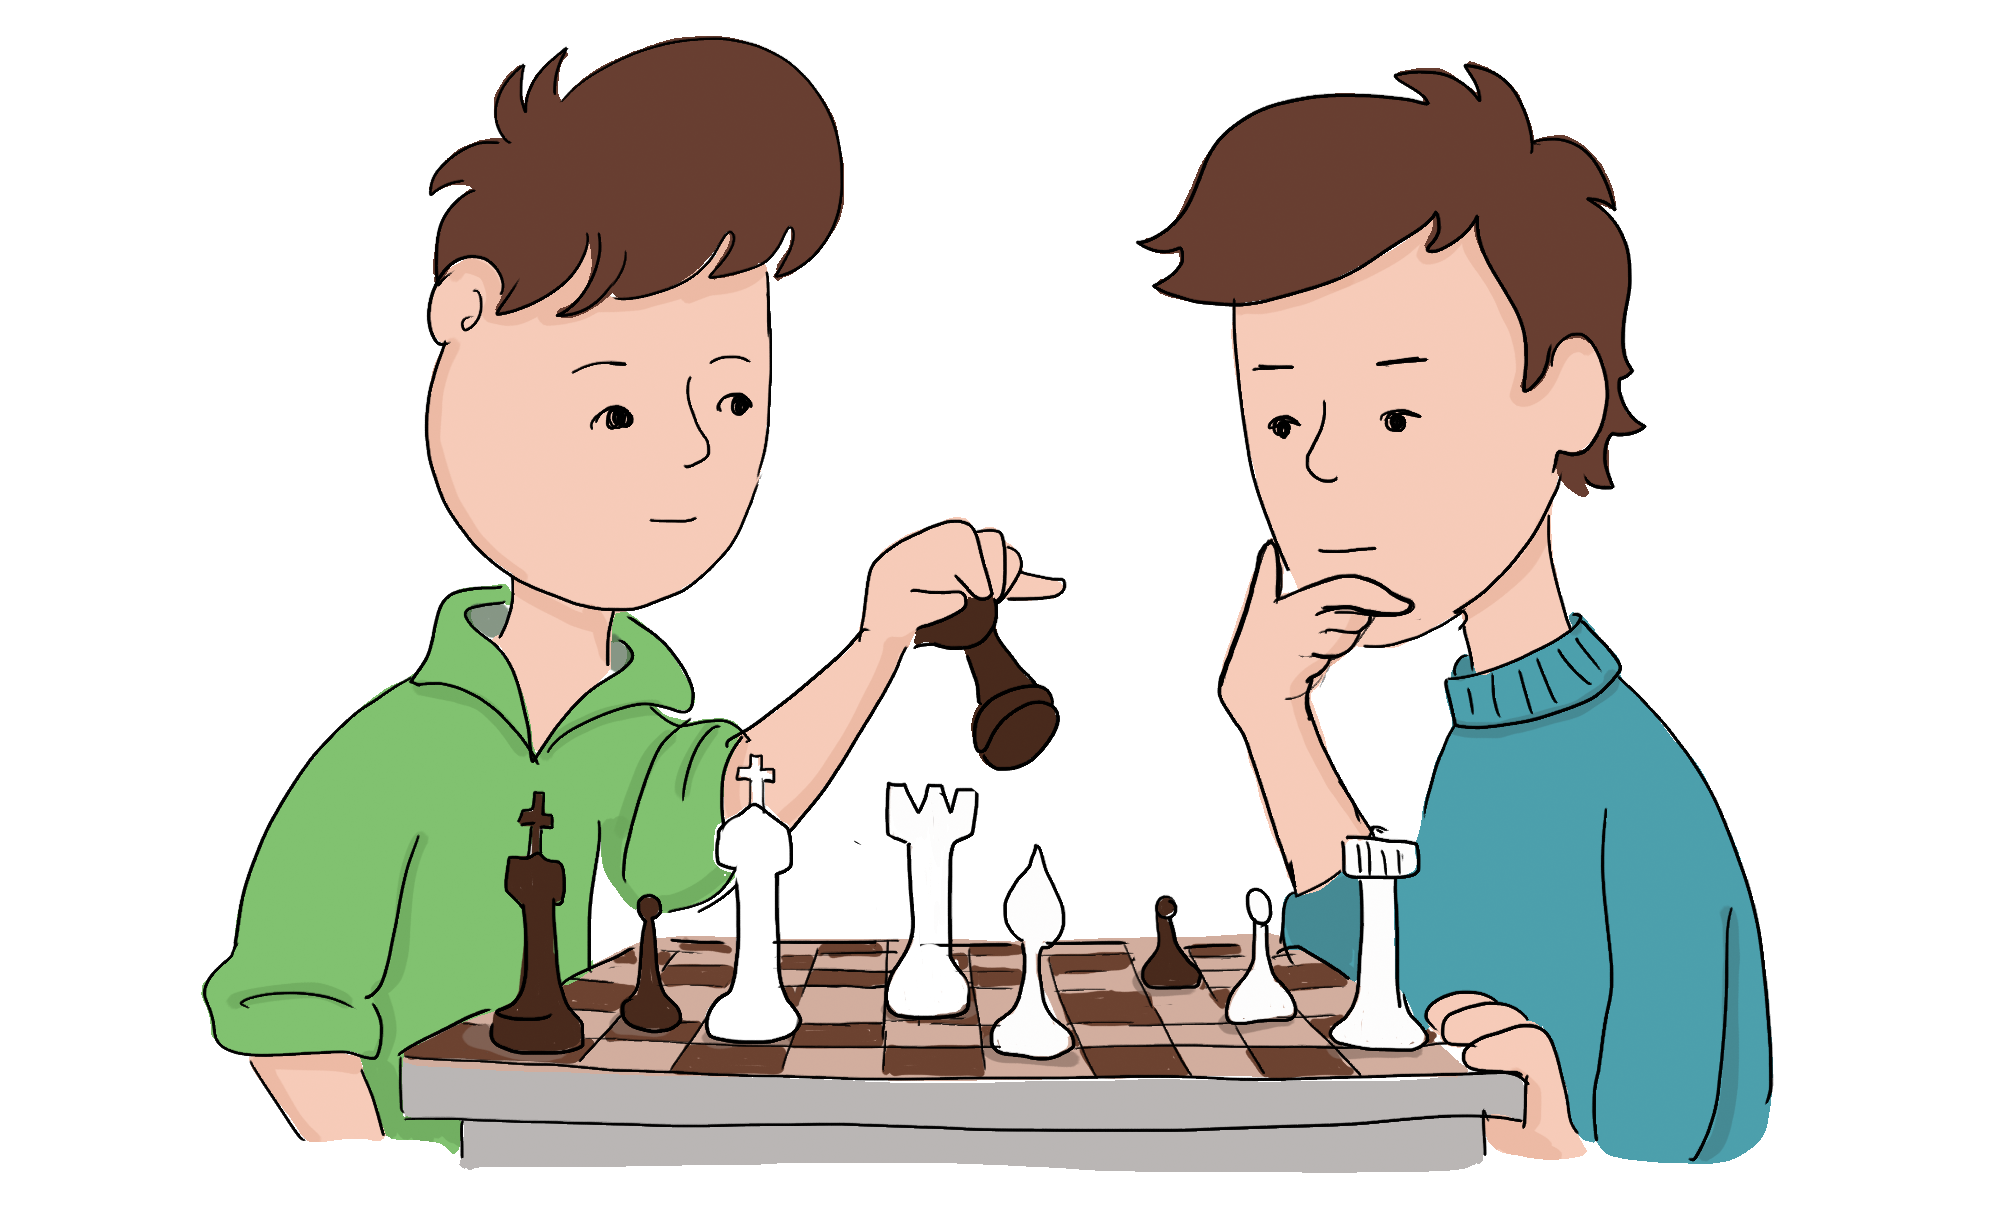
\includegraphics[width=0.8\linewidth]{Pi1_2_Bai5}
		\vspace*{-10pt}
	\end{figure}
	$\pmb{6.}$ Vào một ngày Chủ nhật nọ, Vinh và người em trai nhỏ tuổi hơn là Minh  đạp hai chiếc xe tới hiệu sách trung tâm cách nhà vài cây số. Tại đó mỗi người chọn mua một cuốn sách quý mà nhóm bạn bè cũ đang bàn luận khen ngợi thường xuyên mấy năm nay trên Facebook. Mỗi người đều lấy tổng tất cả các chữ số của tất cả các trang sách mình đã mua và nhận thấy rằng số đó bẳng năm sinh của mình. Vậy ai  trong số hai anh em Vinh và Minh  đang đi học lớp  bồi dưỡng Toán cho học sinh phổ thông nhỉ?
	\begin{figure}[H]
		\centering
		\vspace*{-10pt}
		\captionsetup{labelformat= empty, justification=centering}
		
\includegraphics[width=1\linewidth]{Pi1_2_Bai6}
		\vspace*{-15pt}
	\end{figure}
\end{multicols}
\vspace*{-15pt}
{\color{toancuabi}\rule{1\linewidth}{0.1pt}}
\begingroup
\AddToShipoutPicture*{\put(112,418){
\includegraphics[scale=1]{../tieude2.pdf}}} 
\centering
\endgroup
\graphicspath{{../toancuabi/pic/}}
\vspace*{70pt}

\begin{multicols}{2}
	$\pmb{1.}$ Một chiếc tàu cao tốc dài $18$ m đi ngang qua một cột cây số trong vòng $9$ giây. Hỏi chiếc tàu đó cần bao nhiêu thời gian để đi qua hết một cây cầu dài $36$ m. 
	\begin{figure}[H]
		\centering
		\vspace*{-10pt}
		\captionsetup{labelformat= empty, justification=centering}
		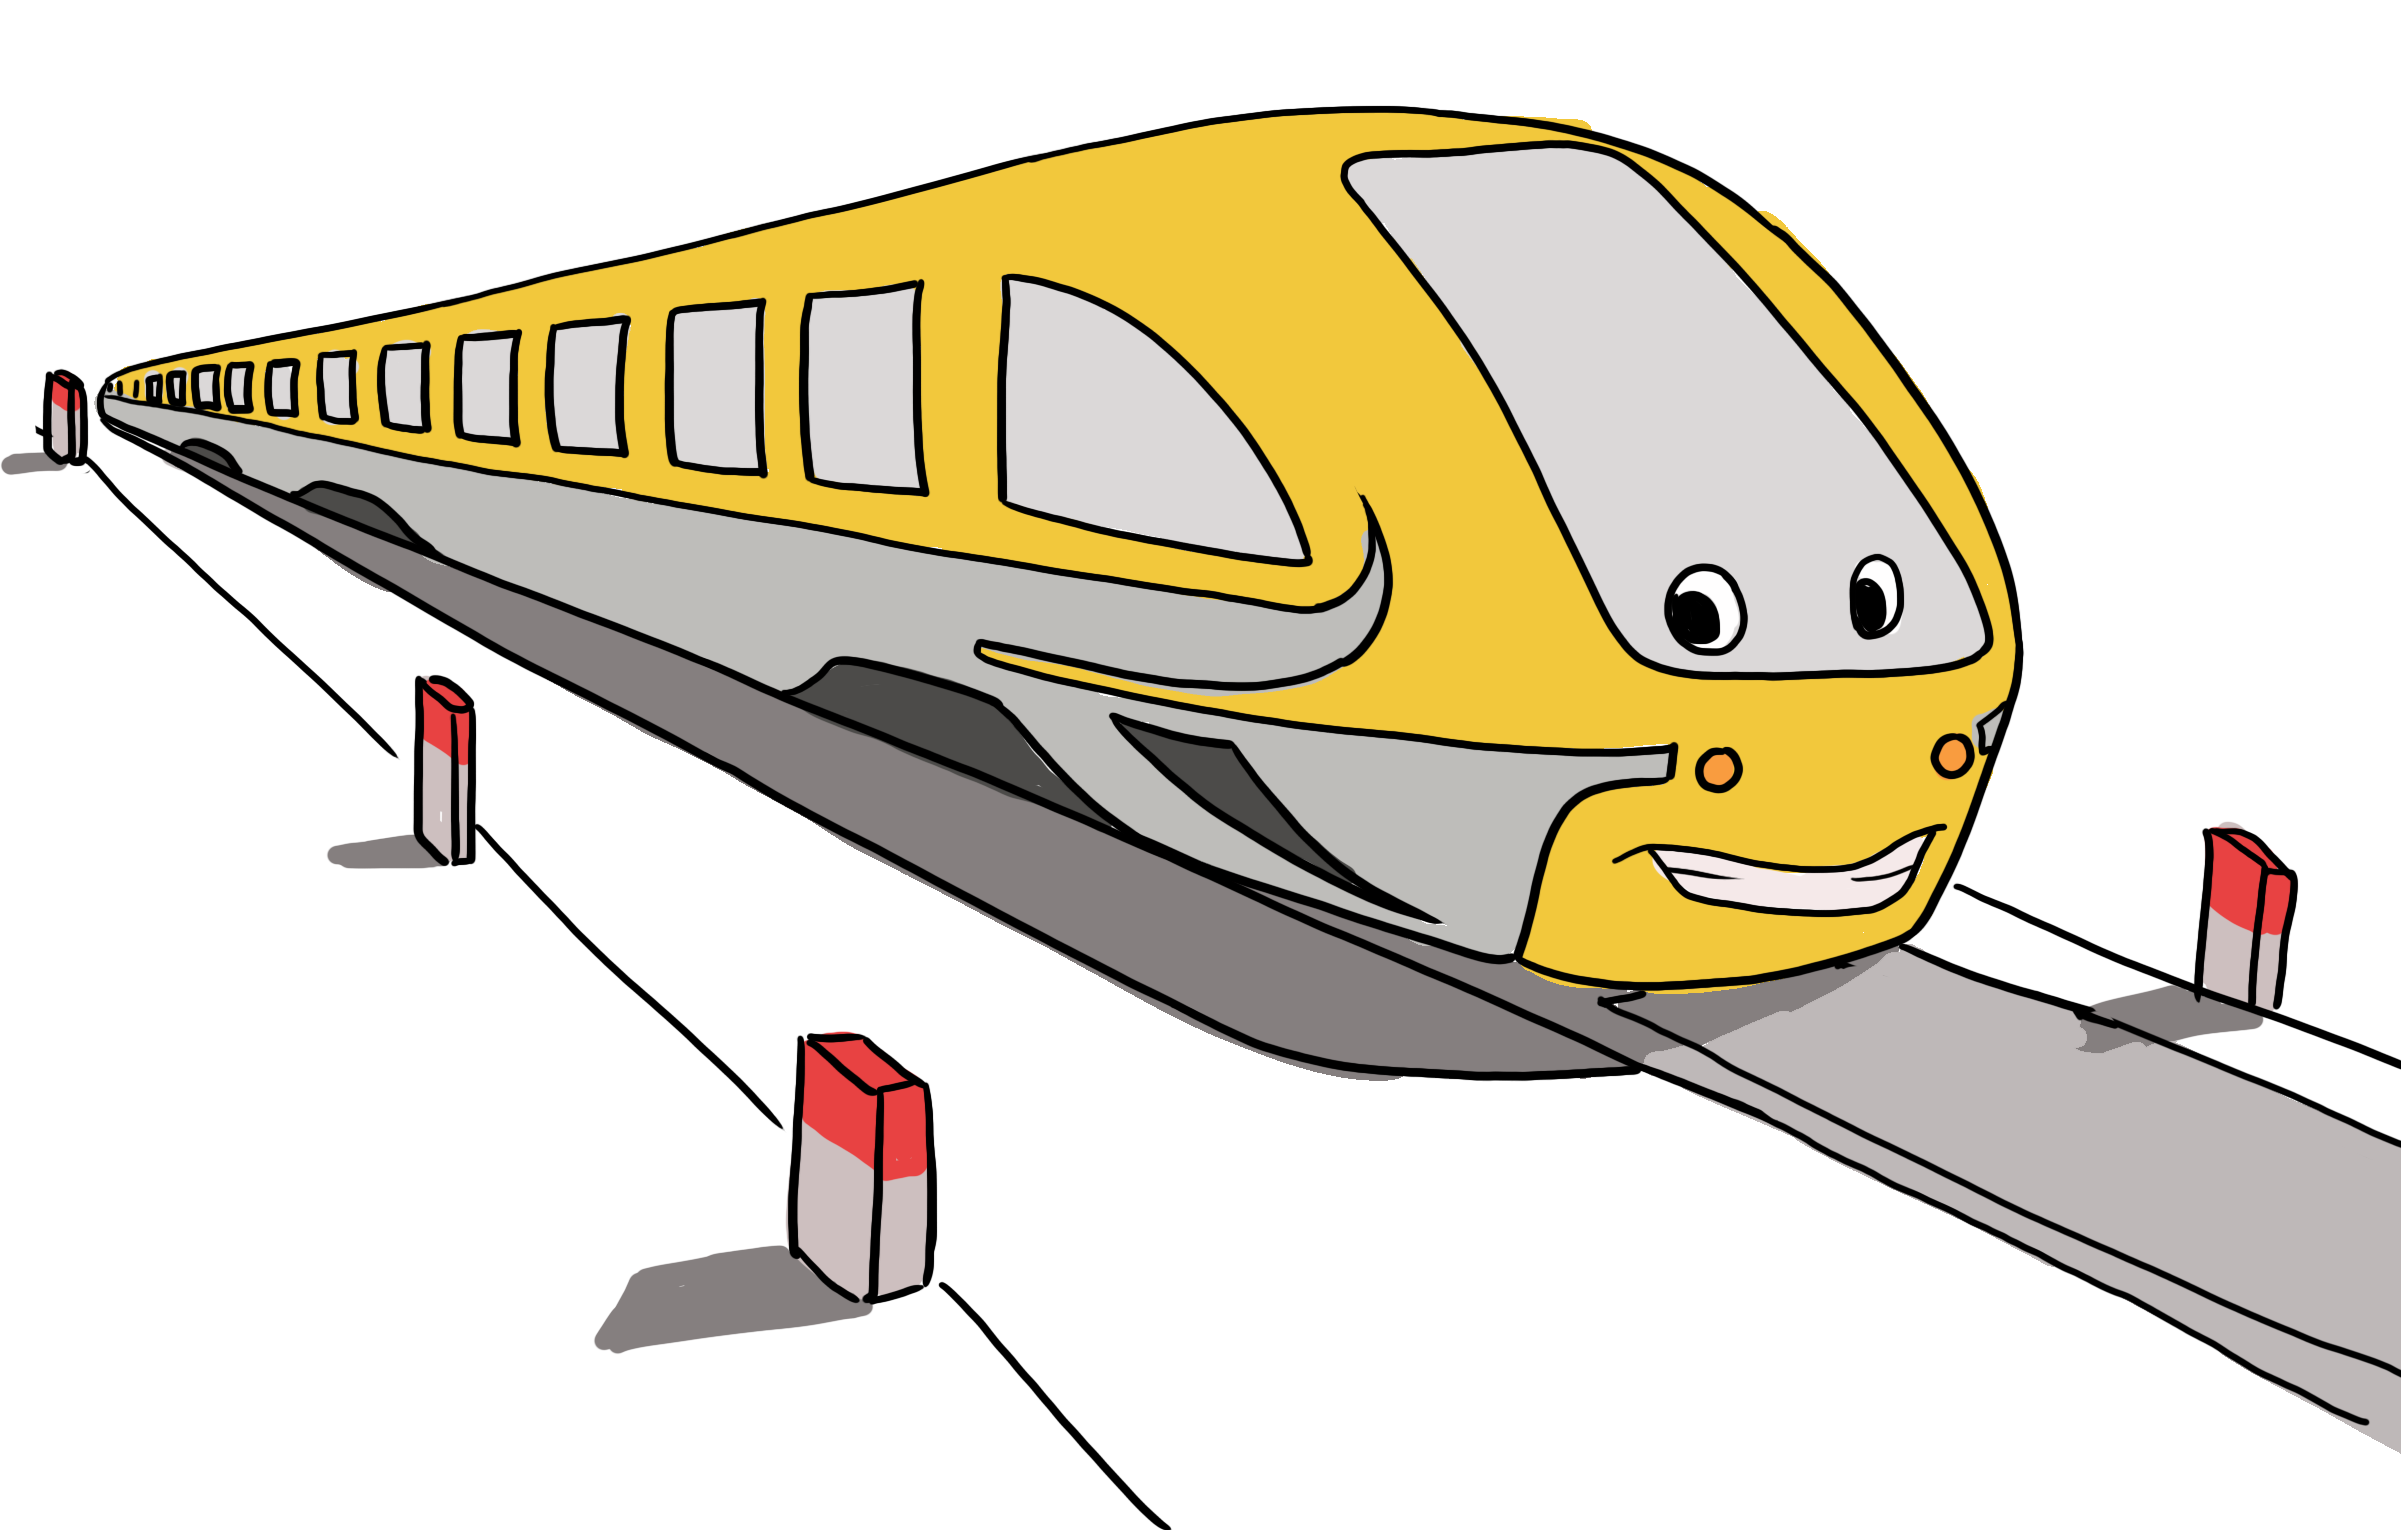
\includegraphics[width=1\linewidth]{Pi10_ToanBi_Bai1}
		\vspace*{-15pt}
	\end{figure}
	\textit{Lời giải.} 	Các em không cần phải tính vận tốc của chiếc tàu cao tốc mà vẫn có thể tìm ra đáp số đúng là $27$ giây. Thật vậy, thời gian tính từ khi đầu tàu đi tới cầu cho tới khi đuôi tàu đi hẳn vào cầu là $9$ giây. Sau $9$ giây đó, đầu tàu đi được đúng nửa cây cầu (do độ dài của tàu bằng nửa độ dài của cầu), và vì thế nó cần thêm $9$ giây để đi hết chiếc cầu. Đuôi tàu cũng cần thêm $9$ giây nữa để đi qua hết cầu. Vì thế tàu cao tốc cần tổng cộng $9+9+9= 27$ (giây) để đi qua hết cây cầu.
	\vskip 0.1cm
	$\pmb{2.}$ Hai cậu bé đi bán cam để gây quỹ xây dựng thư viện. Mỗi cậu có $30$ quả cam. Cậu thứ nhất bán  $10{.}000$ đồng hai quả cam, cậu thứ hai bán $10{.}000$ đồng ba quả cam. Trong lúc đang chuẩn bị bày cam ra bán thì một cậu bị gọi về nhà nên cậu ta nhờ cậu thứ hai bán hộ số cam của mình. Tất cả số cam còn lại được cậu bé thứ hai bán với giá $20{.}000$ đồng năm quả. Nếu như số cam bán riêng như dự định lúc đầu thì đã thu được là $150{.}000$ đồng và $100{.}000$ đồng, tức là tổng cộng có $250{.}000$ đồng, nhưng vì bán gộp $20{.}000$ đồng cho $5$ quả nên  hai cậu chỉ thu được $240{.}000$ đồng. Hỏi số tiền bị hụt $10{.}000$ đồng đã mất ở chỗ nào?
	\vskip 0.1cm
	\textit{Lời giải.} Ta xếp tổng số cam của cả $2$ bạn thành $2$ loại:
	\vskip 0.1cm
	-- Loại $1$: gồm $10$ phần, mỗi phần gồm $5$ quả;
	\vskip 0.1cm
	-- Loại $2$: $10$ quả còn lại.
	\vskip 0.1cm
	Trong mỗi phần ở Loại $1$, ta bán $2$ quả theo giá của cậu thứ nhất và $3$ quả theo giá của cậu thứ $2$. Như vậy, bán mỗi phần này  thu được $20{.}000$ nghìn và theo cách bán này thì mỗi phần thu được số tiền đúng như cách bán của cả hai kiểu.
	\begin{figure}[H]
		\centering
		\vspace*{-10pt}
		\captionsetup{labelformat= empty, justification=centering}
		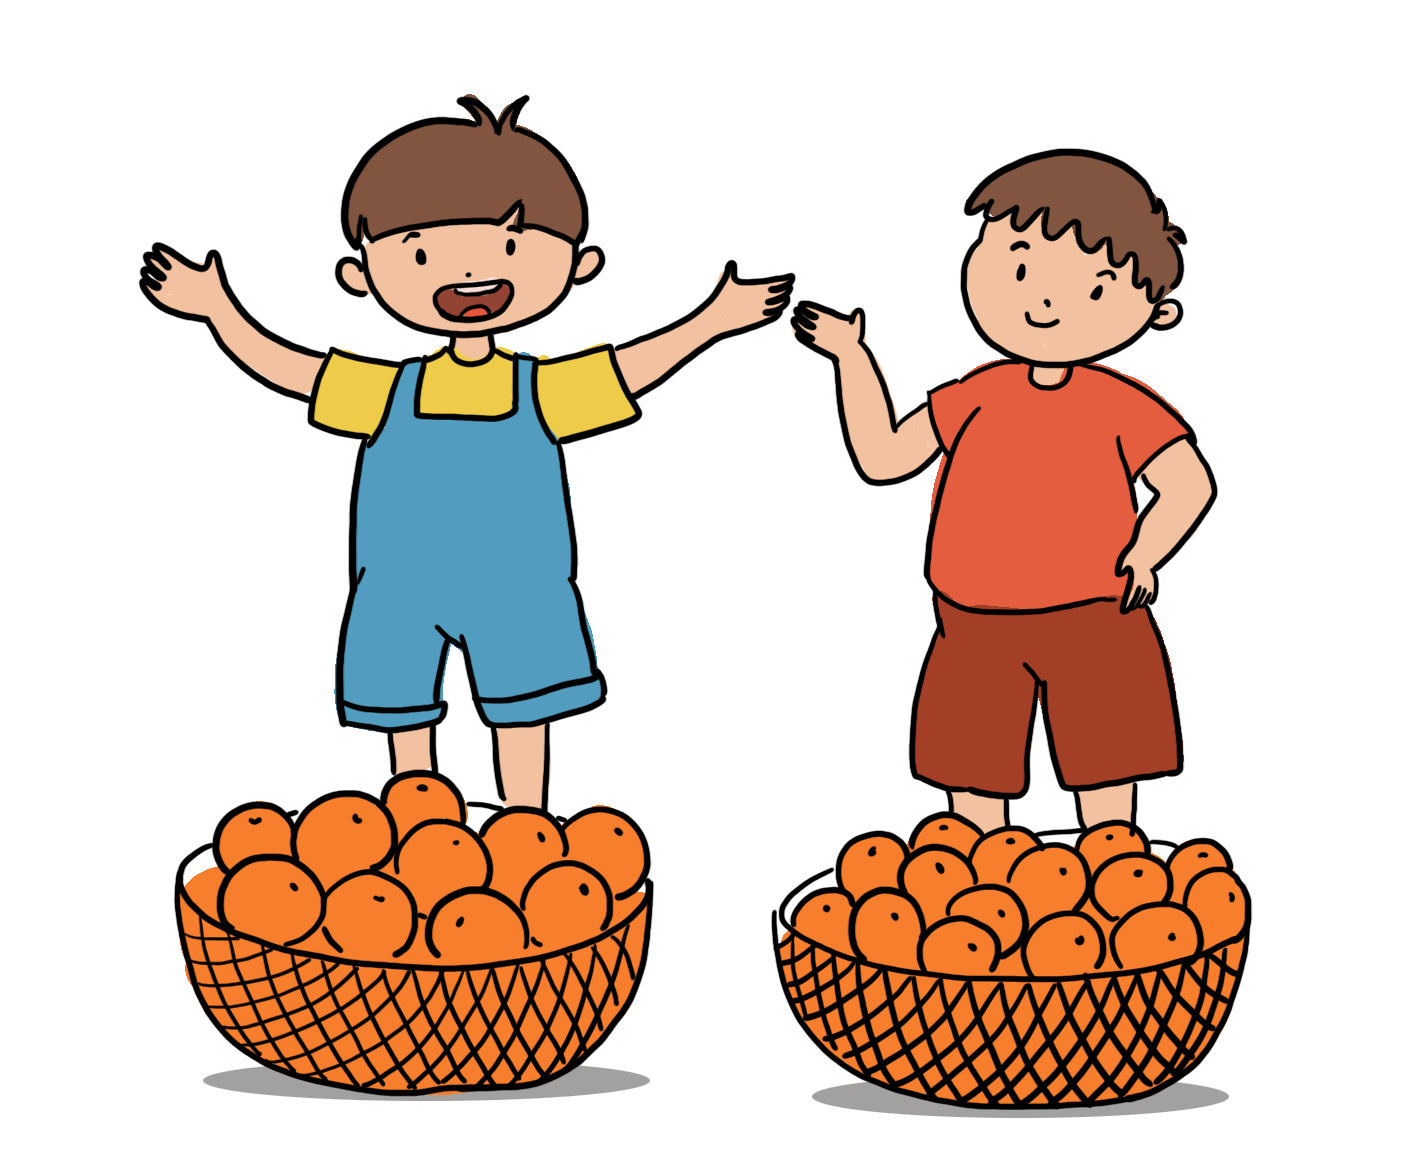
\includegraphics[width=0.7\linewidth]{Pi10_ToanBi_Bai2}
		\vspace*{-10pt}
	\end{figure}
	-- Nếu bán như ban đầu, $10$ quả còn lại sẽ bán theo giá của cậu bé thứ nhất ($10000$ đồng hai quả)
	\vskip 0.1cm
	-- Nếu bán theo cách sau, trong $10$ quả còn lại chỉ có $4$ quả cam được theo giá ban đầu ($10000$ đồng hai quả) và $6$ quả bị bán với giá rẻ hơn ($10000$ đồng ba quả).
	\vskip 0.1cm
	Từ đó theo cách bán sau, số tiền bị thiệt đi là:
	\setlength{\abovedisplayskip}{5pt}
	\setlength{\belowdisplayskip}{5pt}
	\begin{align*}
		6\times\frac{10000}{2} - 6\times\frac{10000}{3} = 10000.
	\end{align*}
	\textit{Cách giải khác.}
	\vskip 0.1cm
	Theo cách bán ban đầu: mỗi quả cam của cậu thứ nhất có giá là: $\dfrac{10000}{2}$ đồng, mỗi quả cam của cậu thứ hai có giá là: $\dfrac{10000}{3}$ đồng.
	\vskip 0.1cm
	Theo cách bán sau thì giá của mỗi quả cam là $\dfrac{20000}{5}$ đồng.
	\vskip 0.1cm
	Như vậy, cứ $2$ quả cam thì bán theo cách sau bị thiệt:
	\begin{align*}
		\dfrac{10000}{2} + \dfrac{10000}{3} - 2\times\dfrac{20000}{5} = \dfrac{1000}{3}.
	\end{align*}
	Vậy khi bán $60$ quả cam thì theo cách sau, cậu bé thứ hai bị mất đi số tiền là:
	\begin{align*}
		30\times \dfrac{1000}{3} = 10000 \text{ (đồng)}
	\end{align*}
	$\pmb{3.}$ Có ba người bạn tập trung lại để đi cắm trại và họ chỉ có duy nhất một chiếc xe máy có $2$ chỗ ngồi. Liệu họ có thể vượt được quãng đường dài $60$ km tới nơi cắm trại sau khoảng thời gian $3$ giờ đồng hồ được hay không, biết rằng vận tốc của mỗi người đi bộ là $5$ km/giờ và vận tốc của xe máy (có tải hay không có tải) luôn là $50$ km/giờ?
	\begin{figure}[H]
		\centering
		\vspace*{-15pt}
		\captionsetup{labelformat= empty, justification=centering}
		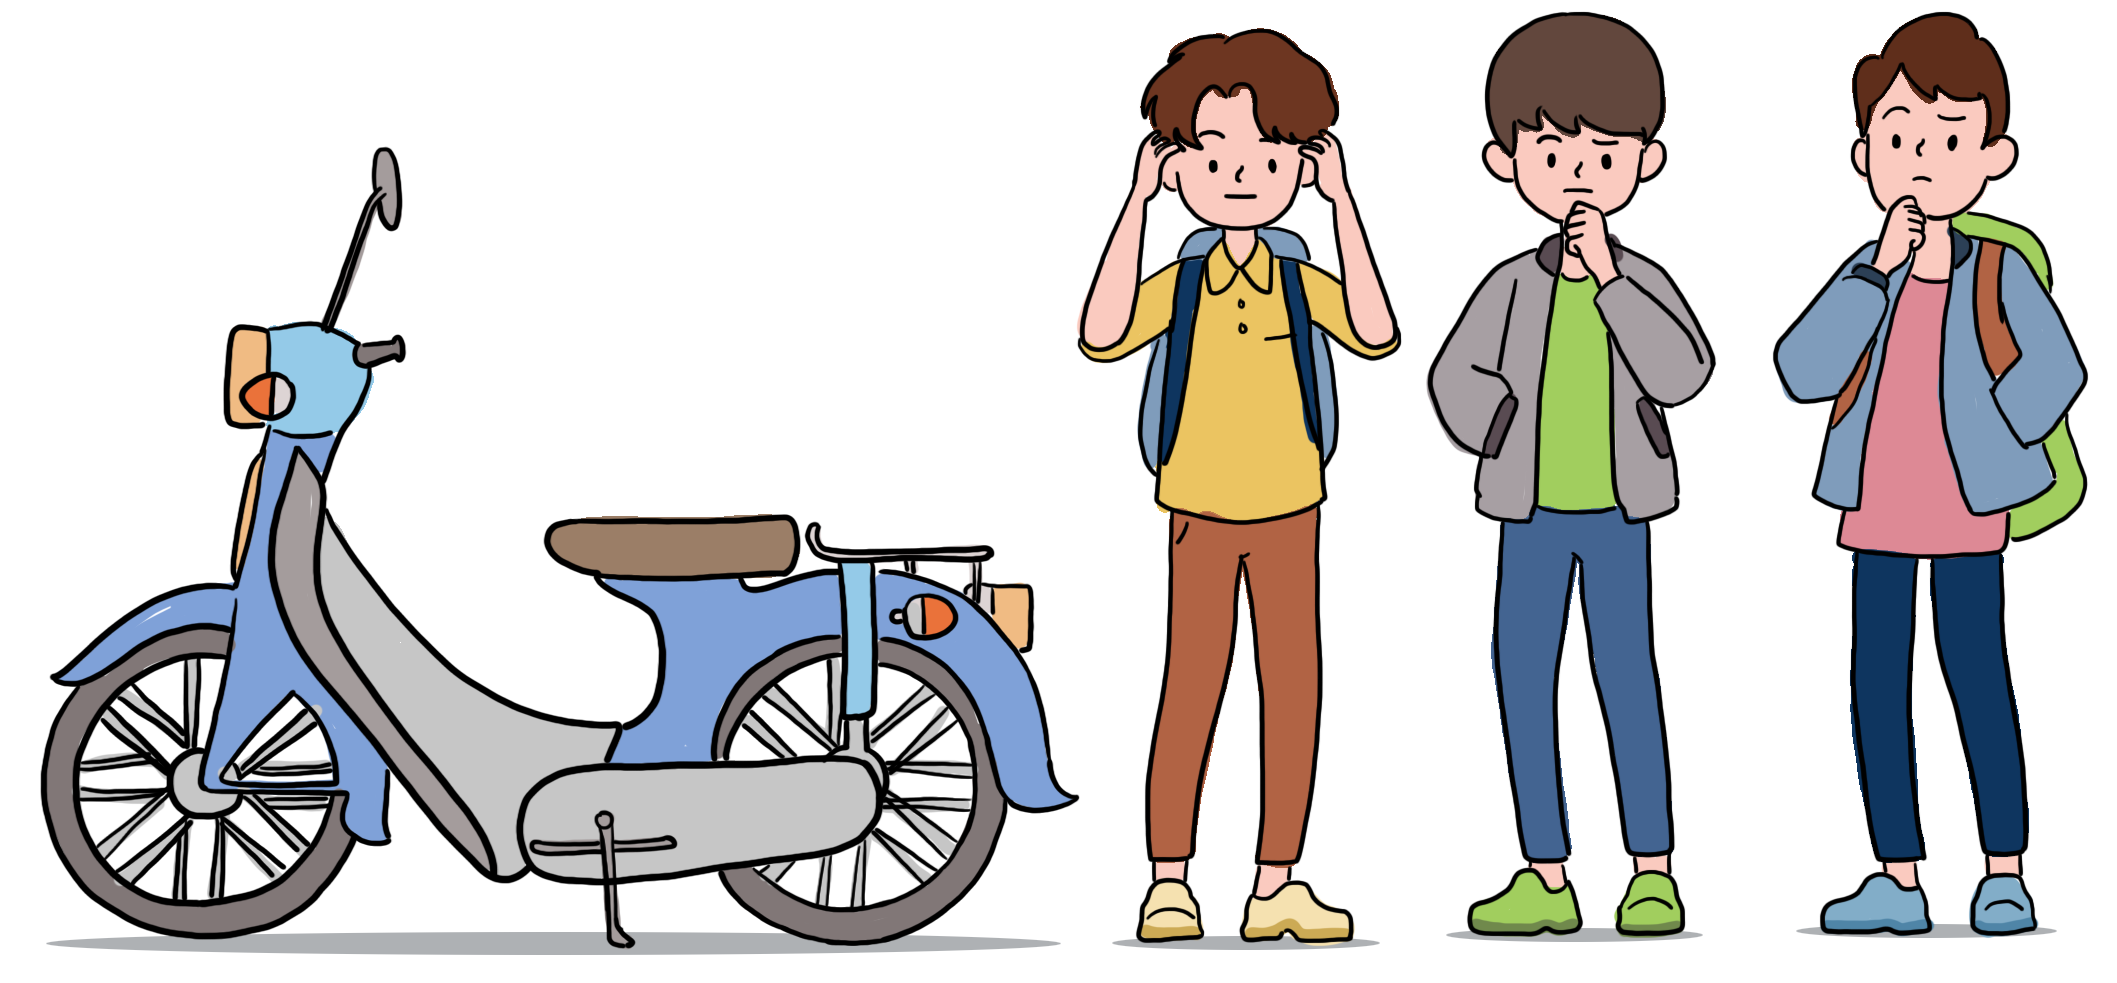
\includegraphics[width=0.95\linewidth]{Pi10_ToanBi_Bai3}
		\vspace*{-15pt}
	\end{figure}
	\textit{Lời giải.} 	Ta gọi $3$ người đó là $A$, $B$, $C$. Trước tiên $A$ sẽ chở $B$ đi bằng xe máy và để $C$ tự đi bộ. Sau $1$ tiếng đi được $50$ km, $A$ để $B$ xuống, cho $B$ tự đến nơi cắm trại một mình, và $A$ quay lại đón $C$. Anh $B$ sẽ đi quãng đường còn lại là $60 -50 =10$ (km) sau đúng $2$ giờ. Sau $1$ giờ, $C$ cũng đã đi được $5$ km, vì vậy $A$ sẽ gặp $C$ sau $(50-5):(50+5)= \dfrac{9}{11}$ (giờ). Thời gian để hai anh này từ lúc gặp lại nhau và quay ngược để đến được nơi cắm trại là $\dfrac{9}{11}+\dfrac{10}{50}$ (giờ).
	\vskip 0.1cm
	Như vậy kể từ lúc đi từ nhà, tổng cộng anh $A$ phải đi mất
	\begin{align*}
		1\!\!+\!\!\dfrac{9}{11}\!\!+\!\!  \dfrac{9}{11}\!\!+\!\!\dfrac{10}{50}  \!=\!\! 1\!\!+\!\!\dfrac{101}{55}\!\!<\!\!1\!\!+\!\!\dfrac{110}{55}\!=\!\!3  \text{ (giờ)}.
	\end{align*}
	Vậy ba người bạn có thể đến được nơi cắm trại sau $3$ giờ chỉ với một chiếc xe máy.
	\vskip 0.1cm
	$\pmb{4.}$ Có $100$ chiếc thẻ bài bằng nhựa đánh số từ $1$ tới $100$ lần lượt được xếp thành hàng ngang. Cứ hai chiếc thẻ xếp cách nhau một chiếc thẻ khác đều có thể đổi chỗ được cho nhau. Liệu em có thể đổi chỗ các chiếc thẻ này bằng cách như trên để xếp lại được $100$ chiếc thẻ trên theo thứ tự ngược lại được hay không?
	\begin{figure}[H]
		\centering
		\vspace*{-10pt}
		\captionsetup{labelformat= empty, justification=centering}
		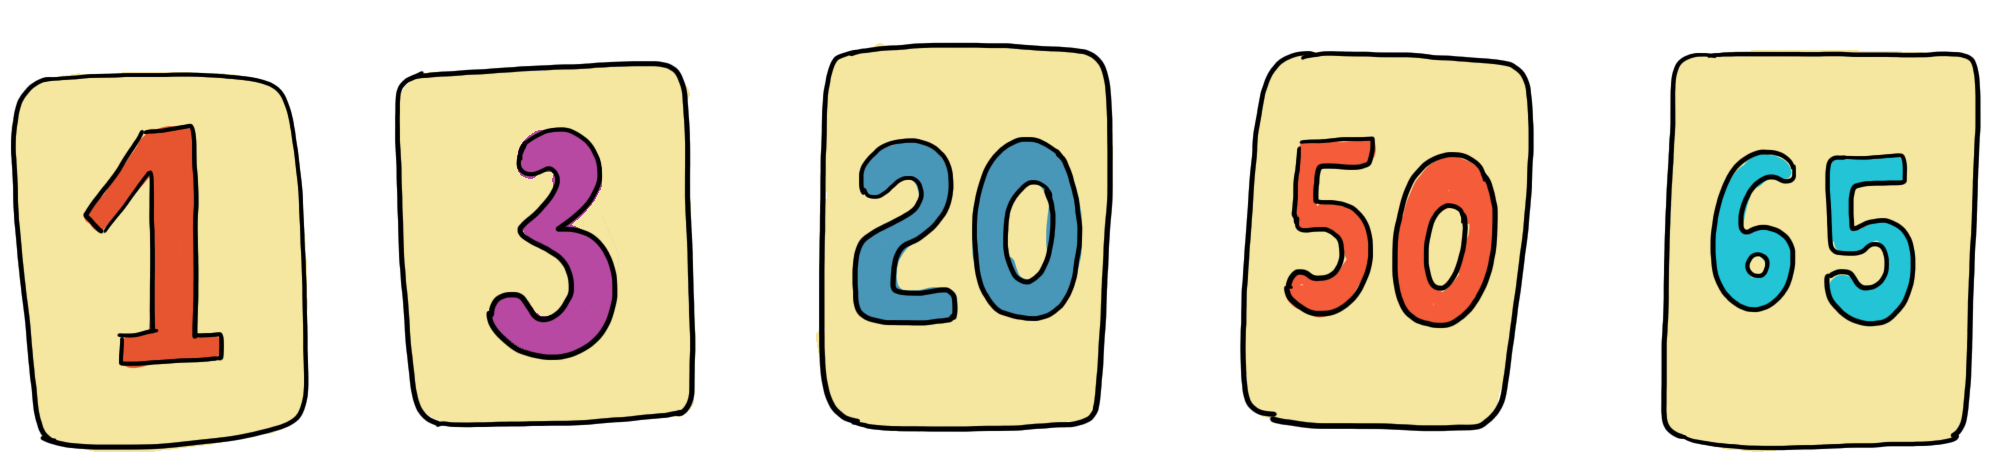
\includegraphics[width=0.98\linewidth]{Pi10_ToanBi_Bai4}
		\vspace*{-10pt}
	\end{figure}
	\textit{Lời giải.} 	Mỗi lần đổi chỗ, một chiếc thẻ sẽ di chuyển vị trí là $+2$ hoặc $-2$ so với vị trí cũ. Như vậy theo cách đổi chỗ như trên, một chiếc thẻ sẽ luôn thay đổi một số chẵn vị trí. Từ vị trí số $1$ tới vị trí $100$ có $99$ vị trí phải thay đổi, đó là một số lẻ. Suy ra ta không thể xếp lại $100$ chiếc thẻ theo thứ tự ngược lại.
	\vskip 0.1cm
	$\pmb{5.}$ Trong ngày khai giảng các bạn học sinh gặp lại nhau sau một mùa hè nên vô cùng mừng rỡ. Gặp lại bạn bè cũ và ai cũng tranh thủ bắt tay bạn mình. Kết thúc màn chào hỏi vui tươi sôi nổi, anh phụ trách thống kê lại trong cuốn sổ các bạn học sinh đã có số lẻ lần bắt tay và tổng cộng có $67$ bạn. Bạn Lâm đứng cạnh anh phụ trách nói nhỏ ``Anh ơi, anh đếm nhầm rồi, chắc chắn không phải là $67$ bạn ạ". Anh phụ trách vô cùng ngạc nhiên, vì sao Lâm lại biết vậy. Em có thể giải thích vì sao Lâm lại cho rằng anh phụ trách đếm nhầm được không?
	\begin{figure}[H]
		\centering
		\vspace*{-10pt}
		\captionsetup{labelformat= empty, justification=centering}
		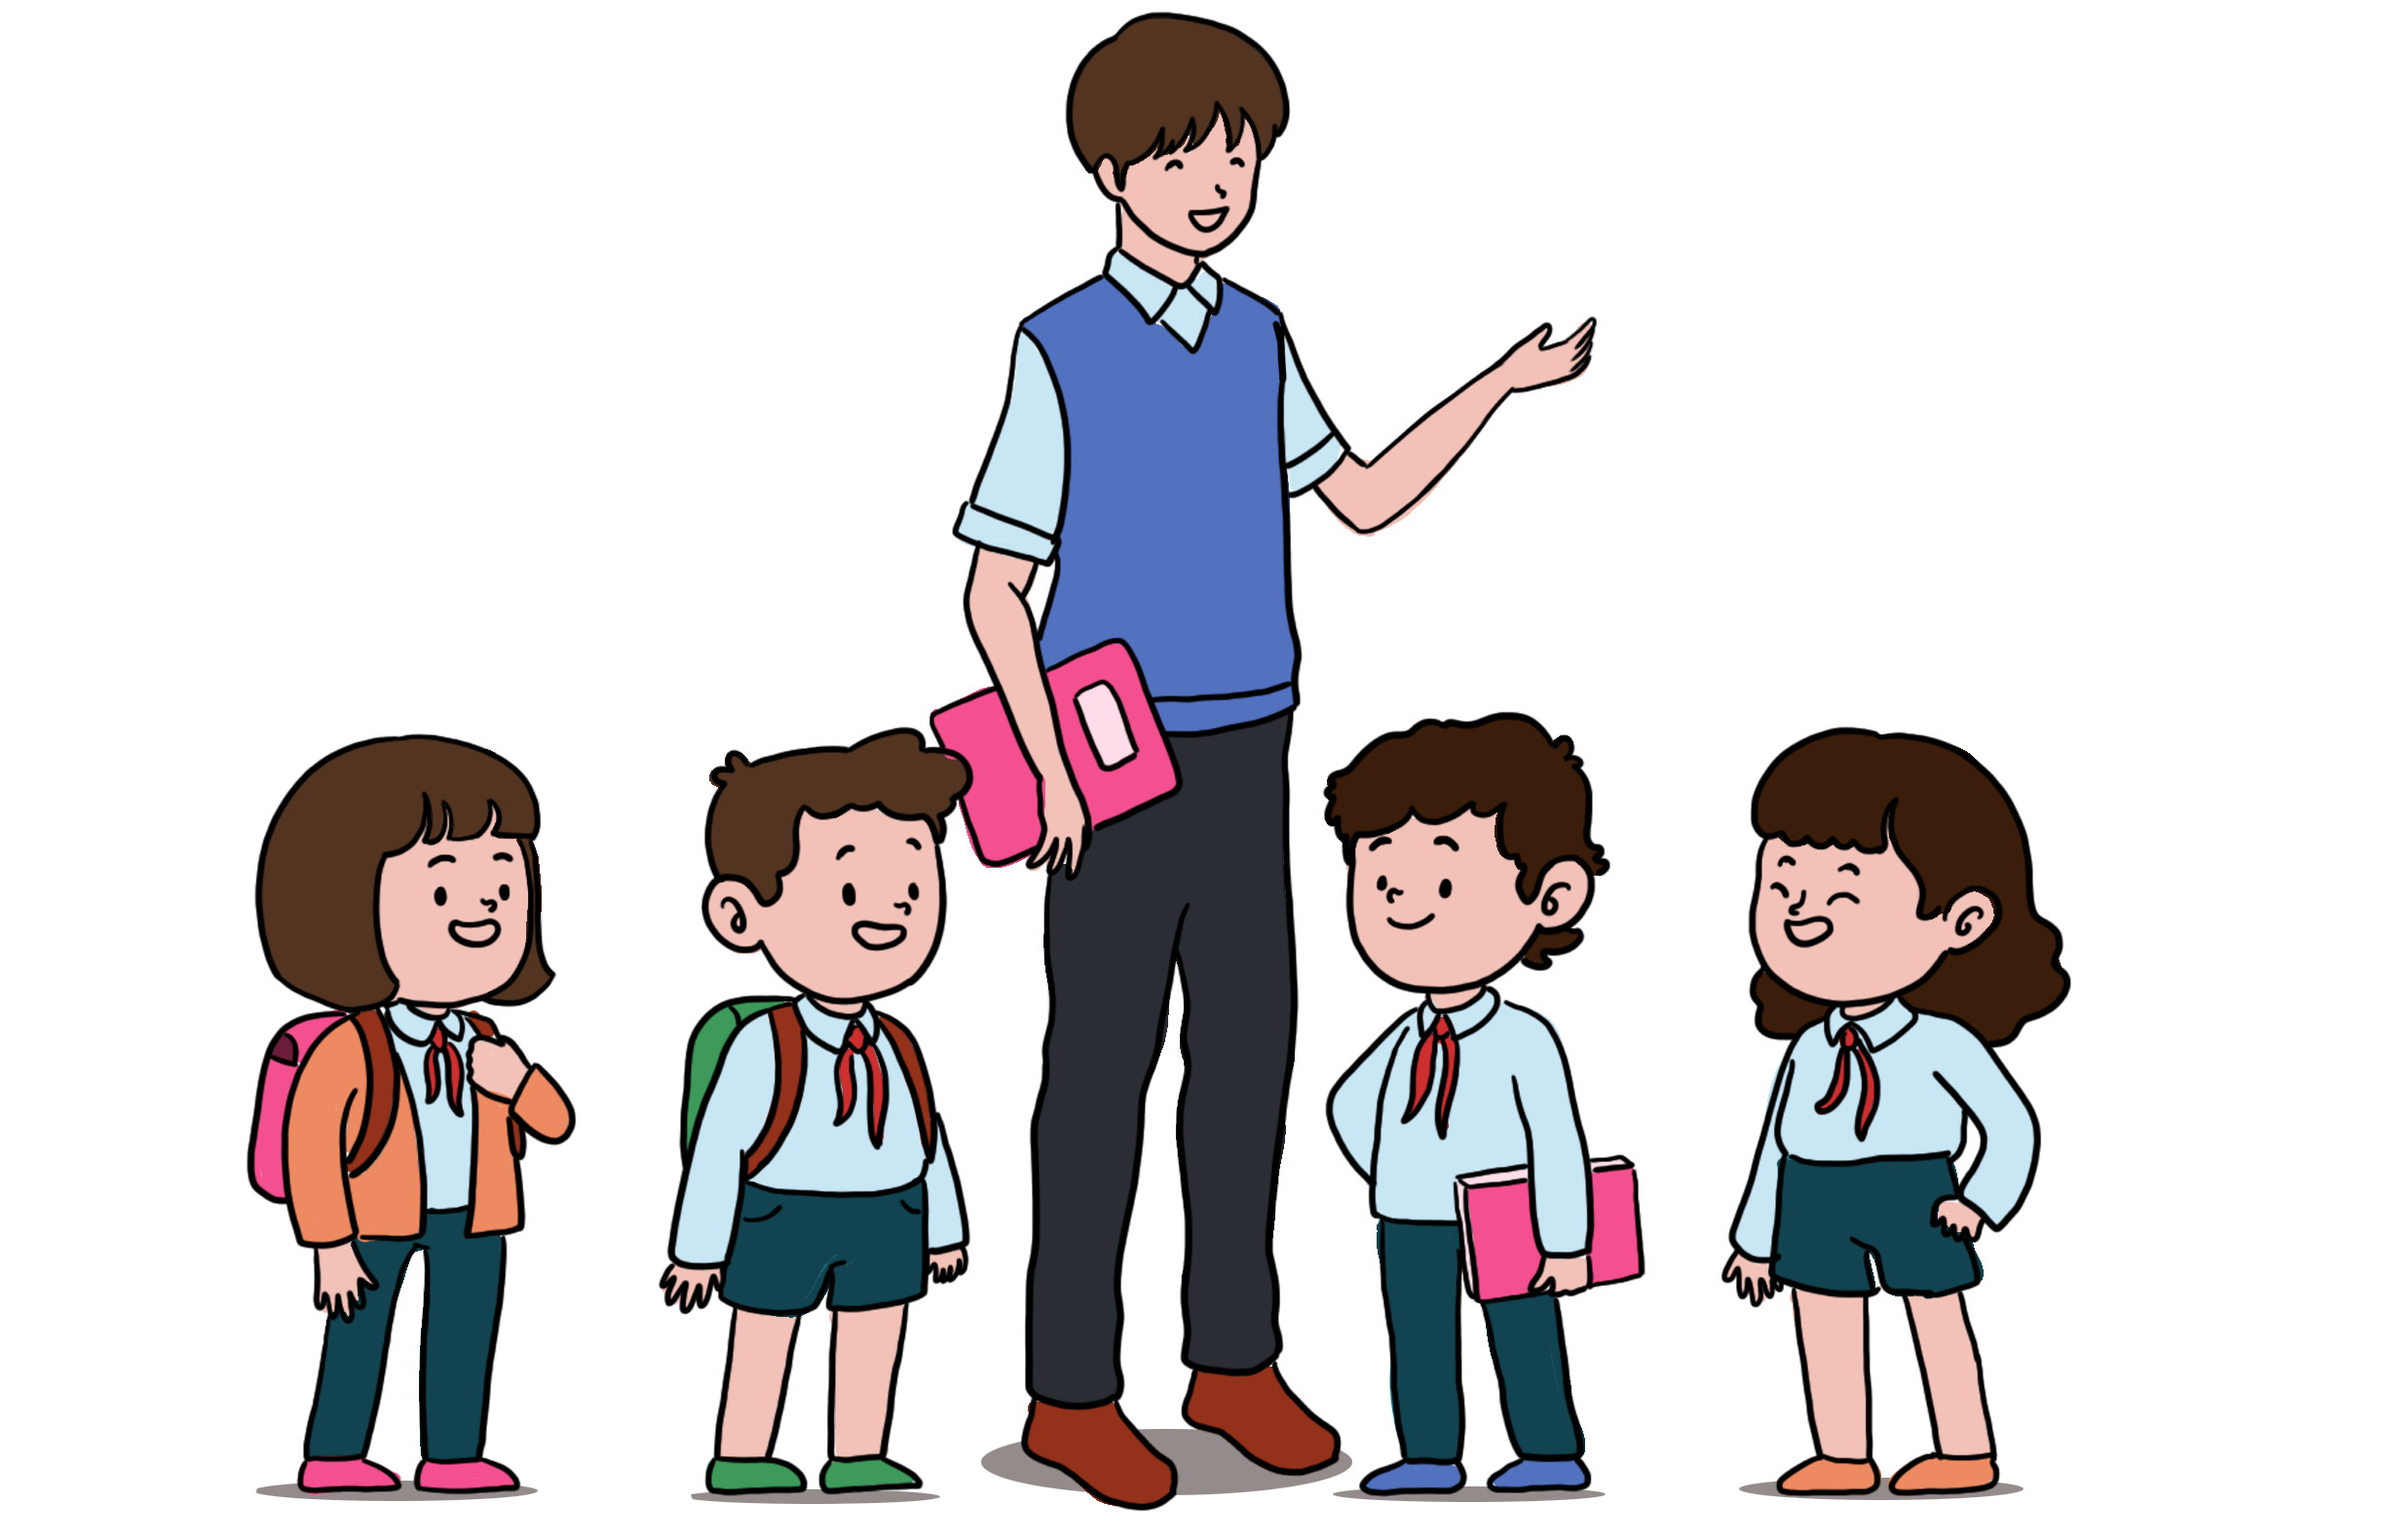
\includegraphics[width=0.9\linewidth]{Pi10_ToanBi_Bai5}
		\vspace*{-10pt}
	\end{figure}
	\textit{Lời giải.} 	Khi một bạn $A$ bắt tay một bạn $B$ của mình, thì $B$ cũng bắt tay $A$, vì thế nếu $P$ là tổng số lượt bắt tay của tất cả các bạn học sinh thì $P= 2+2+\cdots+2=2n$ phải là một số chẵn.
	\vskip 0.1cm
	Ta chia $P$ thành hai tổng. Tổng thứ nhất, ký là $Q$, là số lượt bắt tay của các bạn thực hiện một số chẵn lần bắt tay. Tổng thứ hai, ký hiệu là $R$, là số lượt bắt tay của các bạn thực hiện một số lẻ lần bắt tay. Rõ ràng $P= Q+R$, và $Q$ phải là số chẵn. Vì thế $R = P - Q$ cũng phải là số chẵn. Vì vậy số các bạn có số lẻ lần bắt tay không thể bằng $67$, vì nếu như vậy $R$ sẽ là số lẻ (là tổng của $67$ số lẻ). Do đó Lâm biết được anh phụ trách đã đếm nhầm. Các em cũng có thể thấy từ bài này rằng số các bạn có số lẻ lần bắt tay phải luôn là số chẵn, thú vị phải không nào.
	\vskip 0.1cm
	$\pmb{6.}$ $a)$  Có $50$ vị khách ngồi xung quanh một chiếc bàn tròn được xếp đều, trong số họ có $25$ phụ nữ. Em hãy chứng tỏ rằng có một vị khách ngồi cạnh hai phụ nữ.
	\vskip 0.1cm
	$b)$ Giả sử bây giờ số phụ nữ là $26$ người. Trong buổi tiệc bỗng dưng có hai vị khách làm vỡ mất hai chiếc cốc đặt trước mặt họ. Em hãy chứng tỏ rằng có thể xoay lại chiếc bàn tròn theo một cách nào đó để sao cho hai chiếc cốc vỡ lại đặt trước mặt của hai vị khách~nữ.
	\begin{figure}[H]
		\centering
		\vspace*{-10pt}
		\captionsetup{labelformat= empty, justification=centering}
		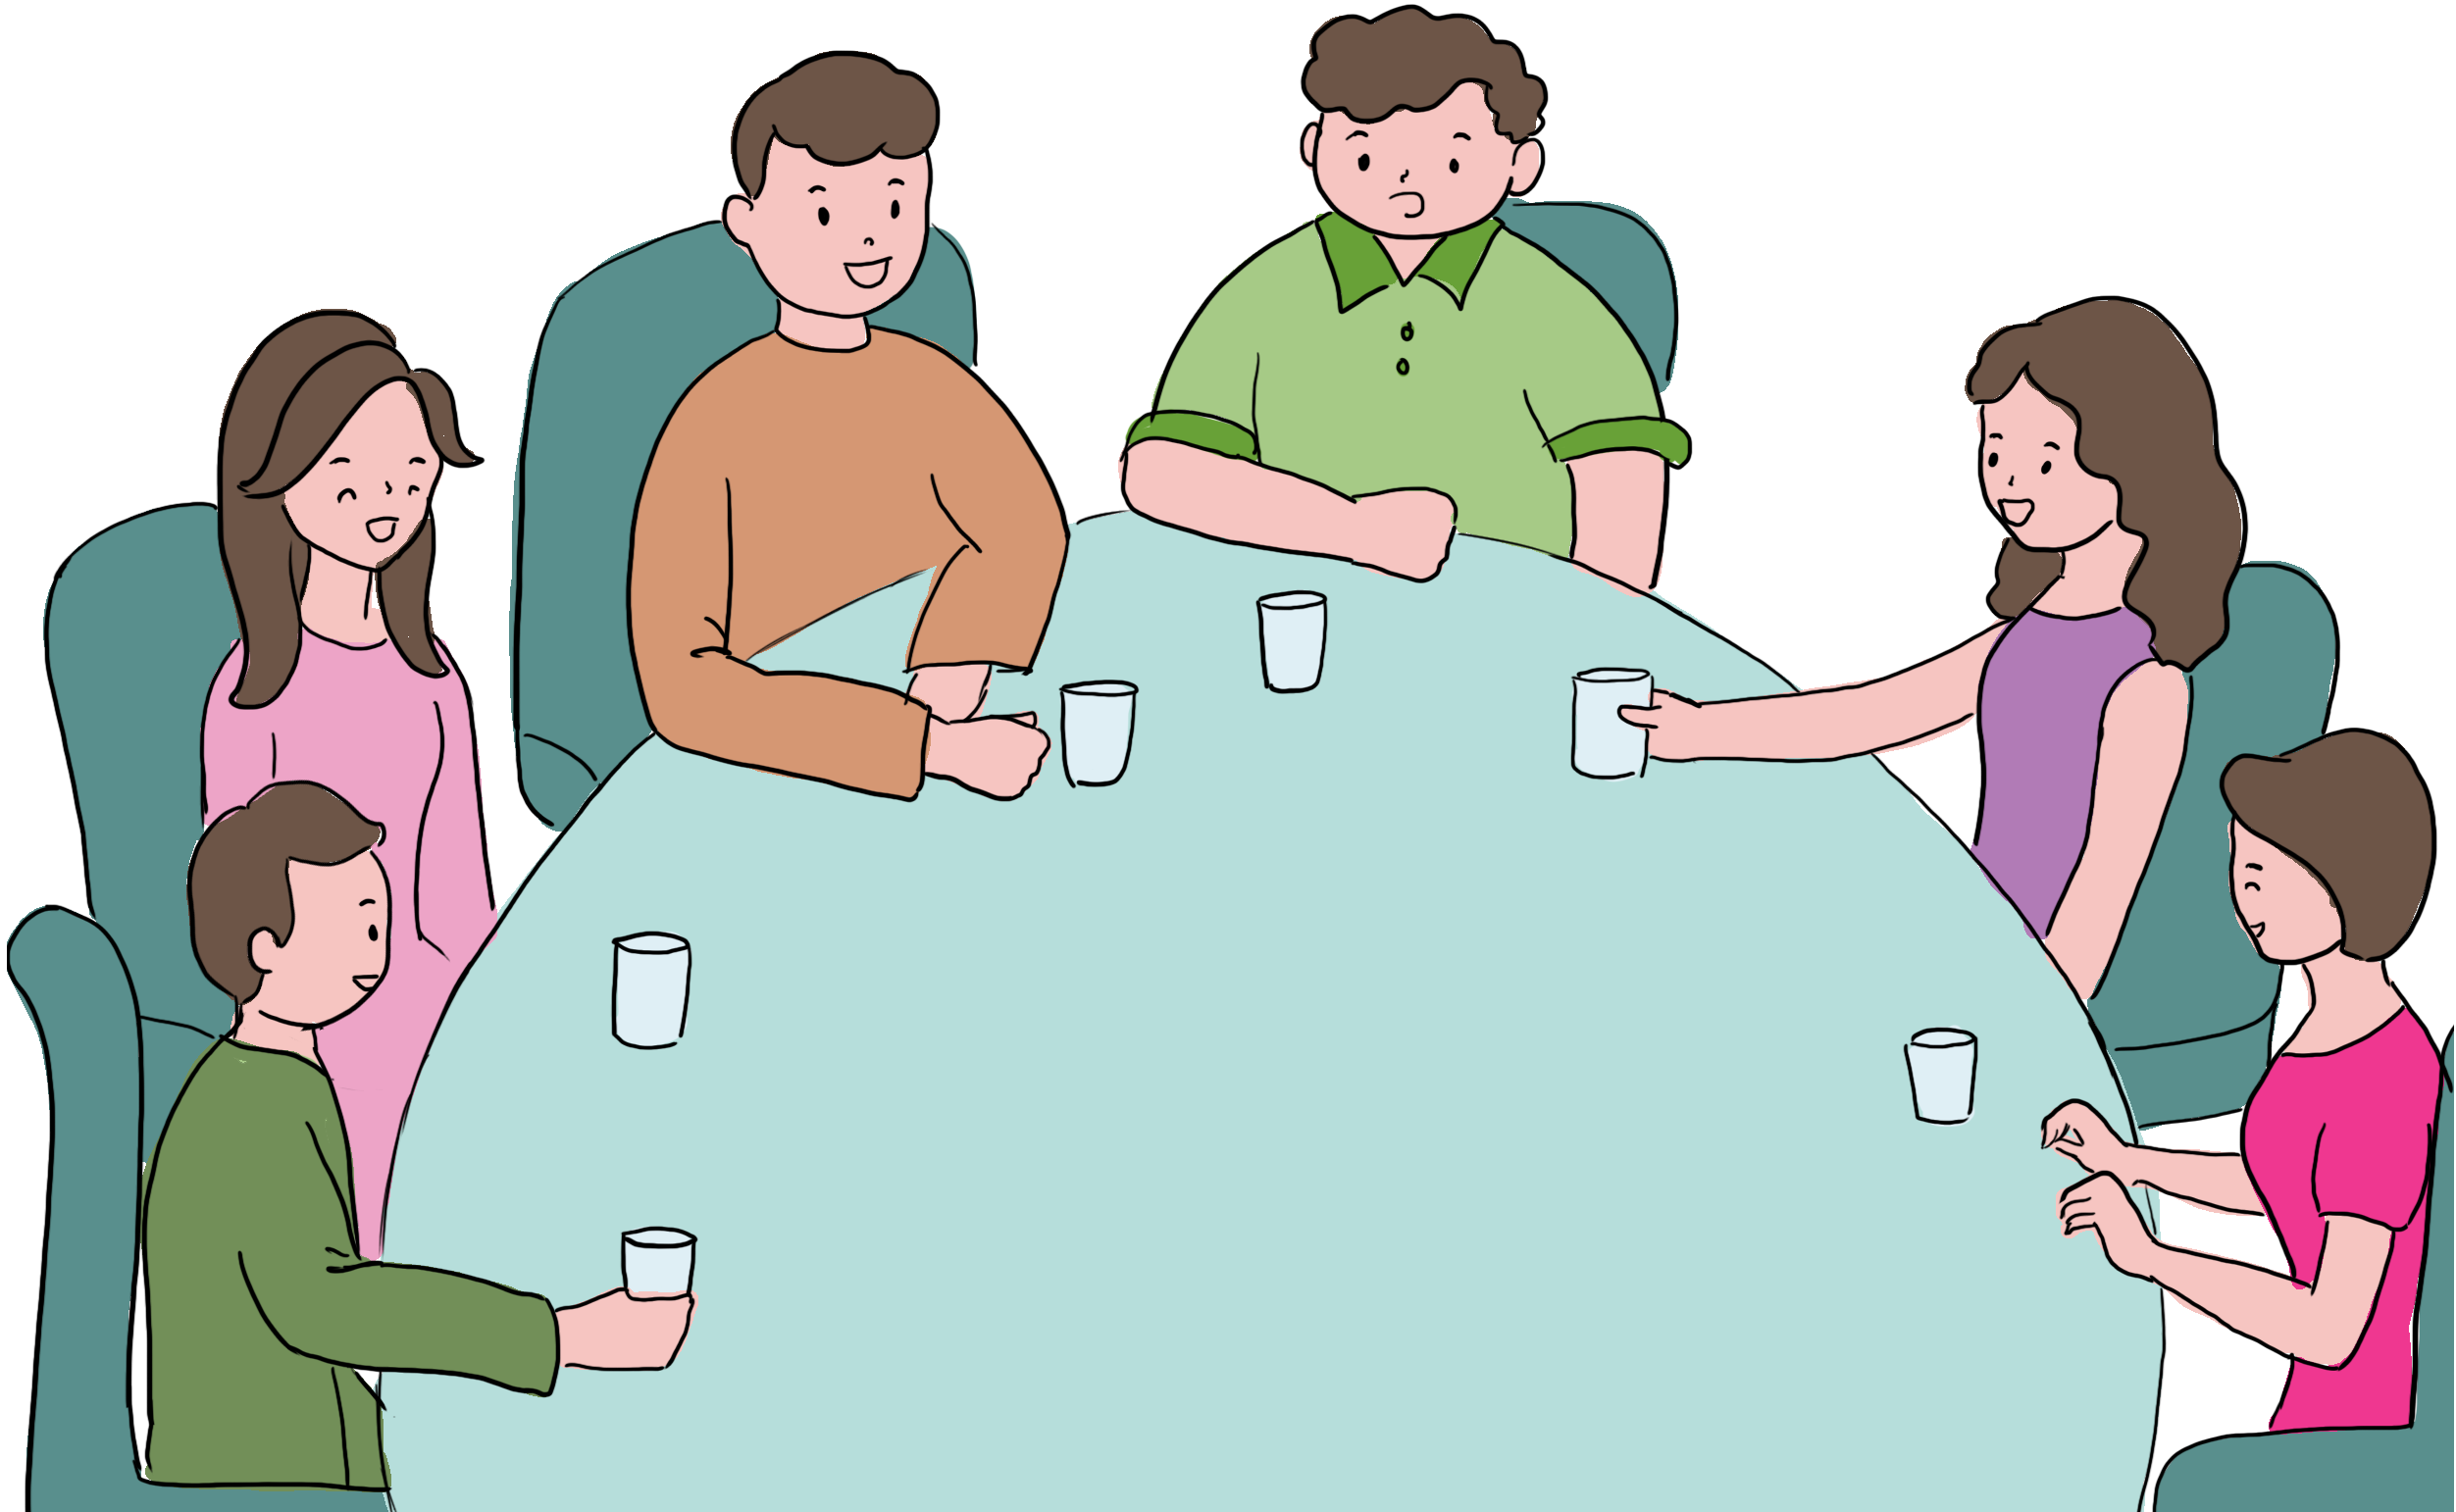
\includegraphics[width=1\linewidth]{Pi10_ToanBi_Bai6}
		\vspace*{-10pt}
	\end{figure}
	\textit{Lời giải.} $a)$	Ta chia hình đa giác $50$ cạnh thành hai hình $25$--giác đều (với các đỉnh xếp đan xen nhau). Do số phụ nữ là $25$ nên theo nguyên lý Dirichlet phải có một trong các hình $25$--giác đều này có ít nhất $13$ phụ nữ ngồi ở các đỉnh của nó. Nhưng do $13>\dfrac{25}{2}$ nên cũng theo nguyên lý Dirichlet, phải có hai phụ nữ ngồi ở hai đỉnh liên tiếp của $25$--giác đều này, vì thế ở giữa họ chỉ có một đỉnh duy nhất của hình $50$--giác ban đầu -- đó chính là vị trí của vị khách cần tìm.
	\vskip 0.1cm
	$b)$ Giả sử hai vị khách làm vỡ cốc ngồi ở hai đỉnh được nối với nhau bởi một đường chéo có độ dài là $a$. Ta sẽ phải tìm hai vị khách nữ cũng ngồi cách nhau một khoảng bằng $a$.
	\vskip 0.1cm
	Nếu $a$ không phải là độ dài của đường chéo lớn nhất, thì từ mỗi một vị khách nữ có tất cả hai đường chéo xuất phát có độ dài $a$. Có tất cả $26\times 2= 52$ đường chéo như vậy. Tuy nhiên số đường chéo có độ dài $a$ chỉ là $50$, vì thế phải có hai đường chéo trong số $52$ đường trên trùng nhau. Ta giả sử đó là đường chéo $AB$. Khi đó $AB=a$, và có hai phụ nữ ngồi tại vị trí $A$ và $B$ là hai vị khách nữ cần tìm.
\end{multicols}
\newpage
\begingroup
\thispagestyle{toancuabinone}
\blfootnote{$^1$\color{toancuabi}Ottawa, Canada.}
\AddToShipoutPicture*{\put(60,733){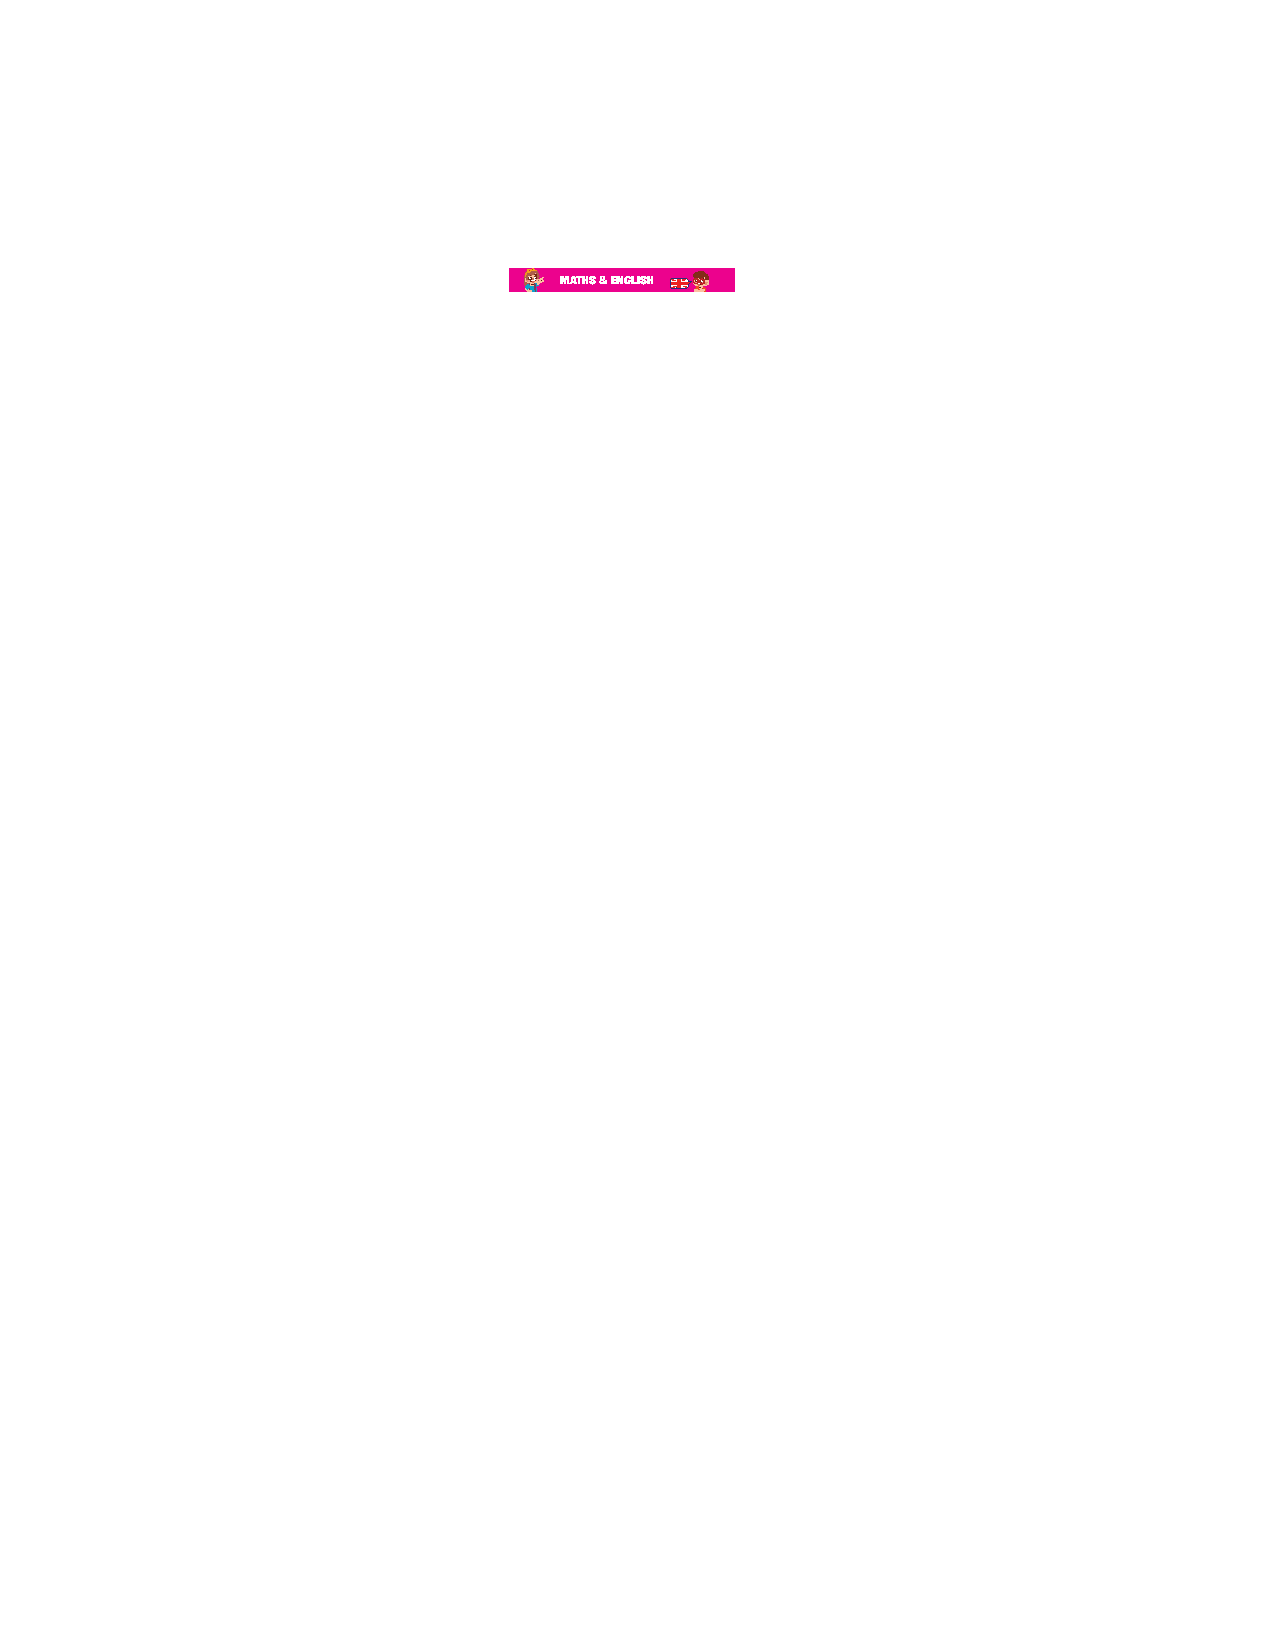
\includegraphics[width=17.2cm]{../mathc.pdf}}}
%\AddToShipoutPicture*{\put(-2,733){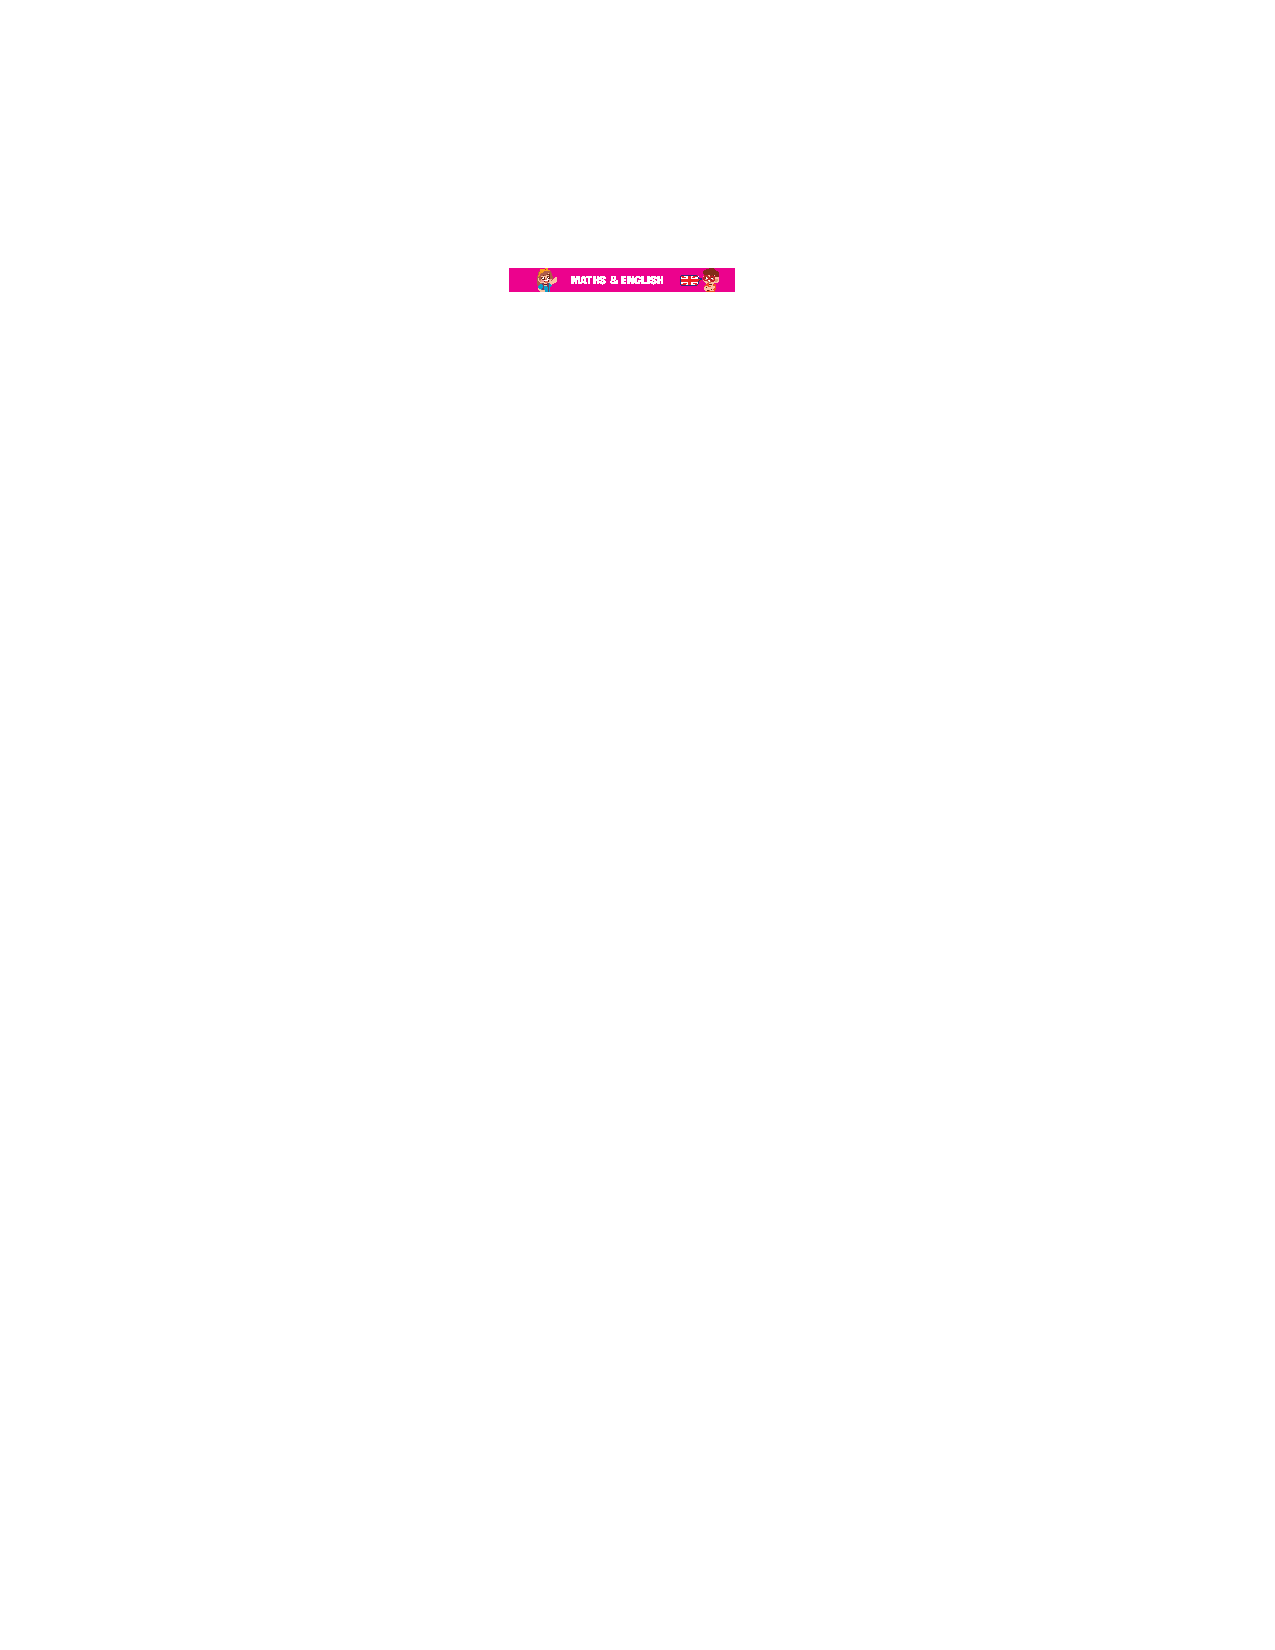
\includegraphics[width=17.2cm]{../mathl.pdf}}} 
\AddToShipoutPicture*{\put(189,675){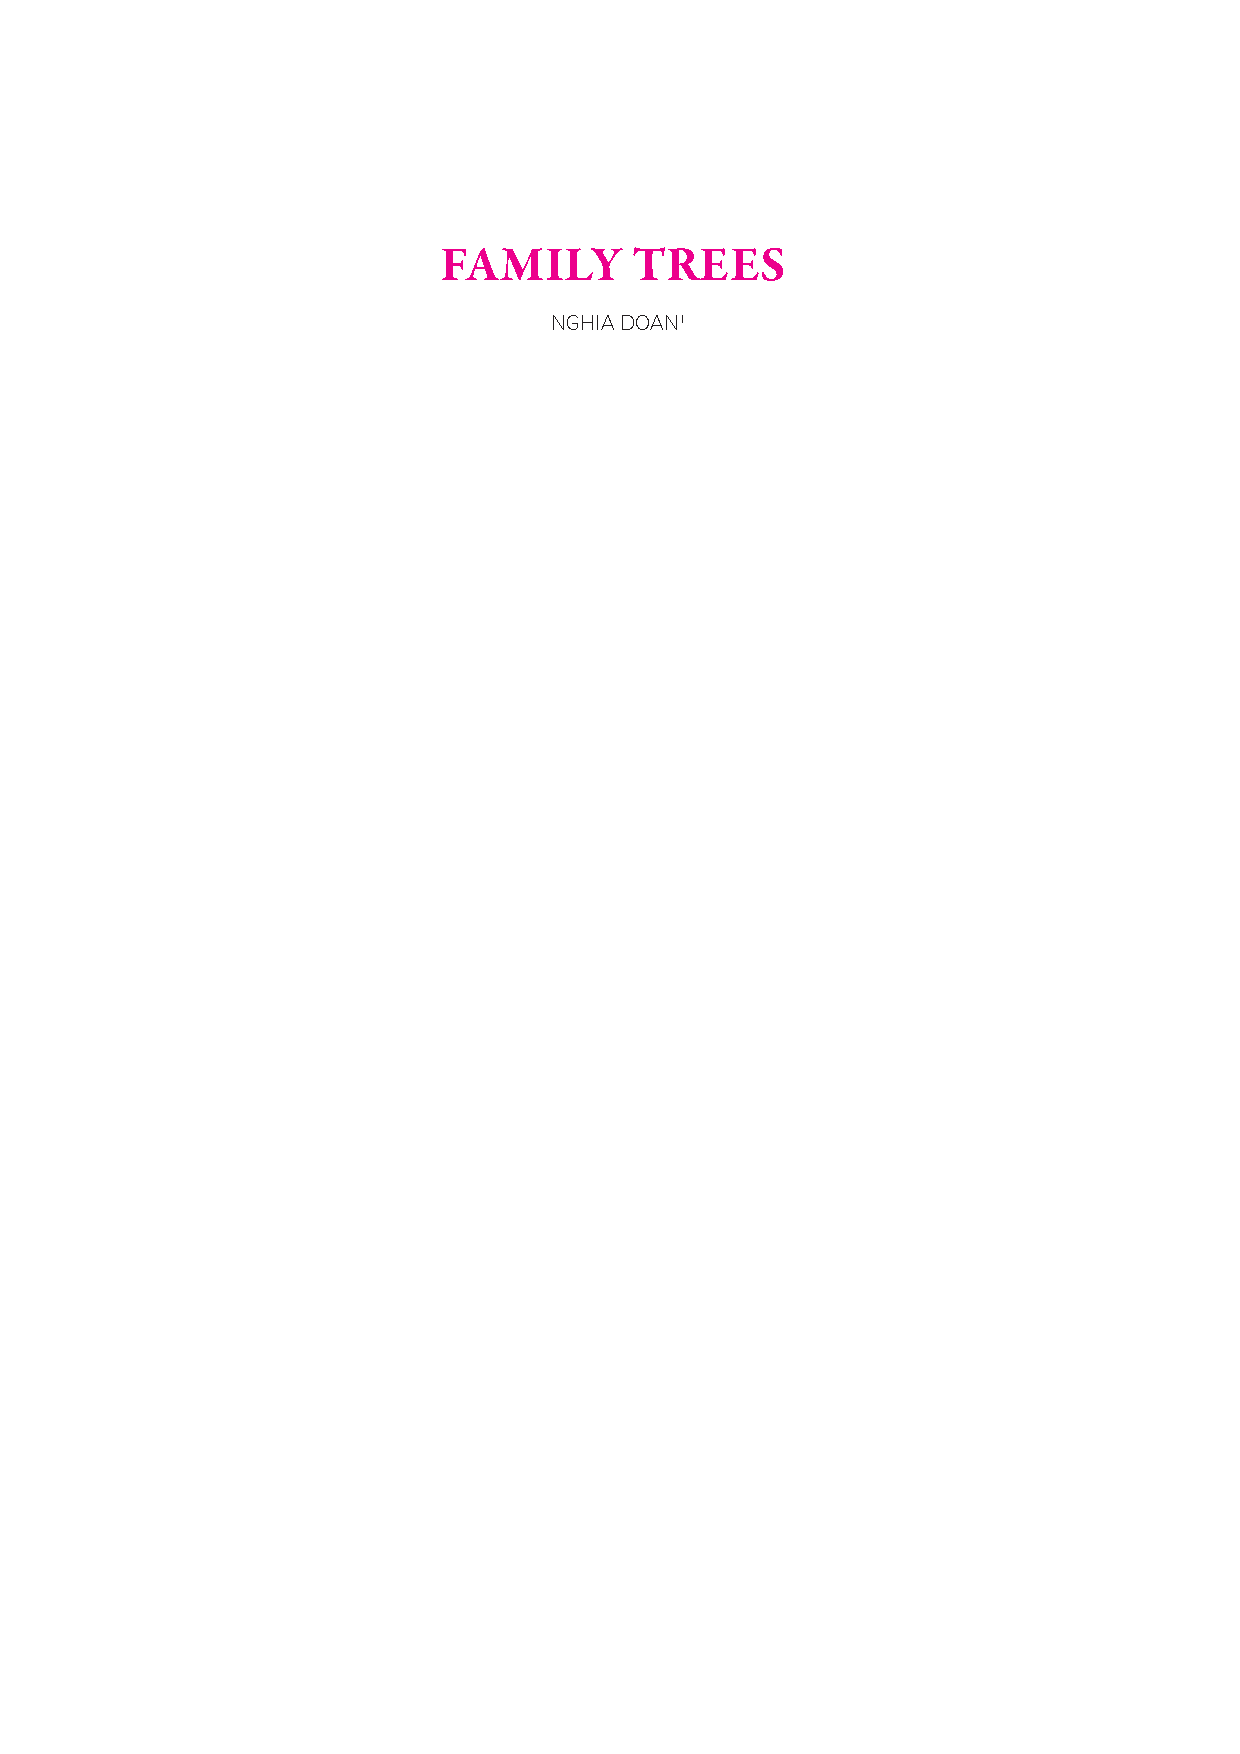
\includegraphics[scale=1]{../tieude4.pdf}}} 
\centering
\endgroup
\graphicspath{{../toancuabi/pic/}}
\vspace*{30pt}

\begin{multicols}{2}
	The diagram below is an example of a \emph{family tree}. The circles denote females and the triangles denote males.
	\begin{figure}[H]
		\vspace*{-5pt}
		\centering
		\captionsetup{labelformat= empty, justification=centering}
		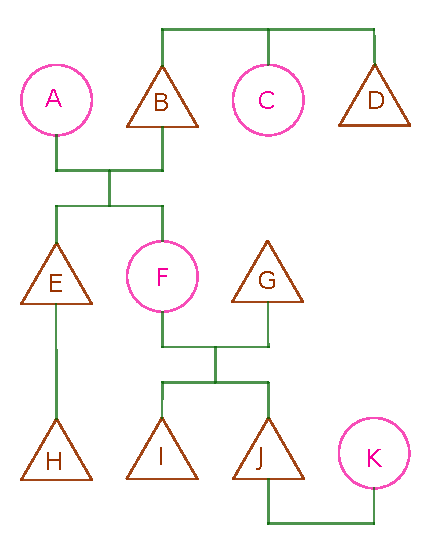
\includegraphics[width= 0.75\linewidth]{hc-2022-2-3-15-1.pdf}
		\vspace*{-10pt}
	\end{figure}
	$A$ and $B$ are married, as are $F$ and $G,$ and $J$ and $K.$
	\vskip 0.1cm
	$B, C,$ and $D$ are siblings, as are $E$ and $F.$
	$E$ and $F$ are children of $A$ and $B.$
	\vskip 0.1cm
	Similarly, the parents of $I$ and $J$ are $F$ and $G.$
	$E$ is the father of $H.$
	\vskip 0.1cm
	In addition, $A$ is the grandmother of $H, I,$ and $J,$
	$F$ is the aunt of $H,$ and $C$ is the sister--in--law of $A.$
	\begin{figure}[H]
		\vspace*{-5pt}
		\centering
		\captionsetup{labelformat= empty, justification=centering}
		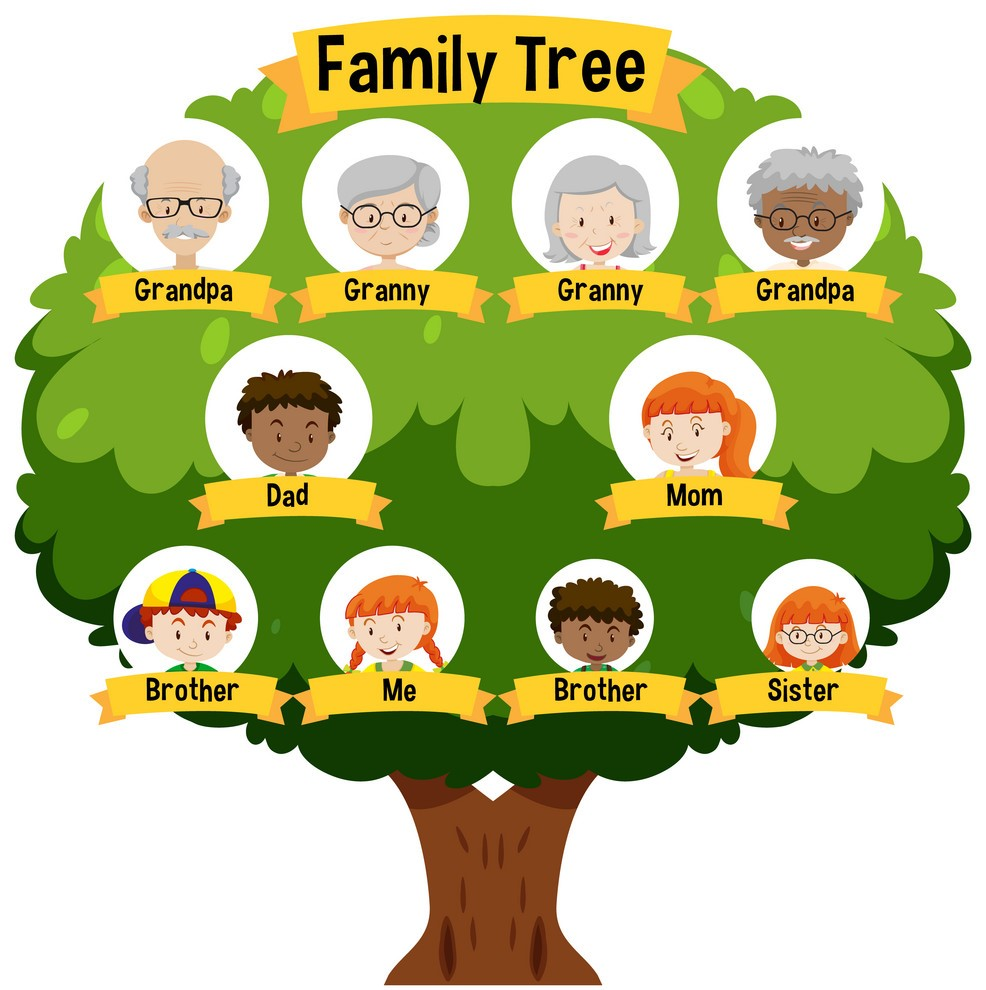
\includegraphics[width= 0.92\linewidth]{tree1}
		%		\vspace*{-5pt}
	\end{figure}
	
	\vspace*{0.1pt}
	
	\vspace*{-7pt}
	\PIbox{
		{\color{toancuabi}\textbf{Example} (Who is who)\textbf{.}}
		Inspector Jade asked six children to briefly introduce their brothers, sisters,
		and first cousins (cousins who share a grandparent). She had to match the name of each child to a numbered position in the family tree with the responses given below. Note that the relations were given in the local language. \emph{Please do not try to guess the genders of the children from the names. It may lead you to wrong conclusions.}
		\vskip 0.1cm
		Response from Binh:
		\vskip 0.1cm
		$\circ$ I have three \textit{arawa}: Kim, Minh, Thao
		\vskip 0.1cm
		$\circ$ I have two \textit{surubu}: Oanh and Yen
		\vskip 0.1cm
		Response from Dinh:
		\vskip 0.1cm
		$\circ$ I have two \textit{surubu}: Oanh and Yen
		\vskip 0.1cm
		$\circ$ I have one \textit{ere}: Binh
		\vskip 0.1cm
		Response from Kim:
		\vskip 0.1cm
		$\circ$ I have one \textit{arawa}: Dinh
		\vskip 0.1cm
		$\circ$ I have one \textit{surubu}: Binh
		\vskip 0.1cm
		Response from Minh:
		\vskip 0.1cm
		$\circ$ I have one \textit{ere}: Yen
		\vskip 0.1cm
		$\circ$ I have two \textit{arawa}: Dinh and Thao
		\vskip 0.1cm
		Response from Thao:
		\vskip 0.1cm
		$\circ$ I have two \textit{surubu}: Yen and Binh
		\vskip 0.1cm
		$\circ$ I have two \textit{arawa}: Minh and Dinh}
	\begin{figure}[H]
		\vspace*{-5pt}
		\centering
		\captionsetup{labelformat= empty, justification=centering}
		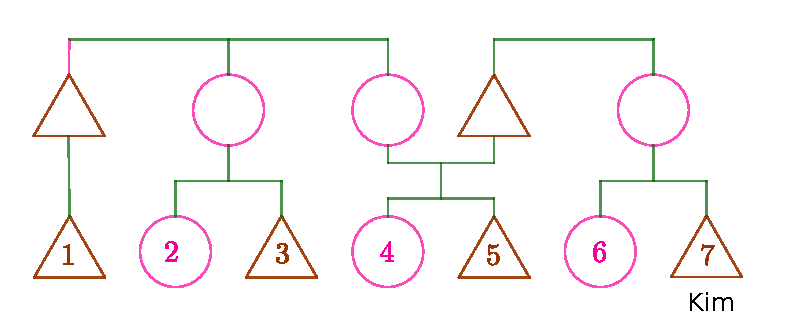
\includegraphics[width= 1\linewidth]{hc-2022-2-3-15-2.pdf}
		\vspace*{-20pt}
	\end{figure}
	\textit{Solution.} From what Binh said, Binh has the same type of relations to three children.
	Consequently, those children cannot be Binh's sisters or brothers,
	and \textit{arawa} does not mean sister or brother.
	Only the child with number $4$ or $5$ has three cousins in the same gender.
	\vskip 0.1cm
	Looking at the cousins of the children with numbers $4$ and $5$, we see that \emph{arawa} and \emph{suburu} refer to the gender of the cousins. Observe that Binh is a \emph{suburu} to Kim and Kim is an \emph{arawa} to Binh. Therefore, Binh and Kim are of opposite genders. Because both children with numbers $4$ and $5$ have three male cousins, Kim has to be a boy and so Binh is a girl. Thus, Binh is the girl with number $4$. 
	\vskip 0.1cm
	Now, Kim, Minh and Thao are the children with numbers $1$, $3$ and $7$; \emph{arawa} means \emph{male cousin}.
	Furthermore, Binh is a \textit{suburu} to Kim and Thao;
	in other words, she is a \textit{female cousin} to them.
	\vskip 0.1cm
	We deduce that Binh is not a \emph{suburu} to the boy with number $5$. Thus, Dinh is the boy with number $5$.
	Obviously, she is not an \textit{arawa} to anyone.
	Since she is an \textit{ere} to Dinh, \emph{ere} means {sister} and Dinh is Binh's brother.
	\vskip 0.1cm
	Next, Thao must be the boy with number $1$ because Thao has two female cousins and two male cousins. It follows that Minh is the boy with number $3$.
	\vskip 0.1cm
	Yen is an \emph{ere} to Minh, so Yen is the girl with number $2$. Finally, Oanh is the girl with number $6$.
	\vskip 0.1cm
	The answer is $1-$Thao, $2-$Yen, $3-$Minh, $4-$Binh, $5-$Dinh, $6-$Oanh, $7-$Kim.
	\vskip 0.25cm
	\PIbox{
		\centerline{\textbf{\color{toancuabi}Vocabulary}}
		\vskip 0.1cm
		{\color{toancuabi}male}: nam
		\vskip 0.1cm
		{\color{toancuabi}female}: nữ
		\vskip 0.1cm
		{\color{toancuabi}family tree}: cây phả hệ 
		\vskip 0.1cm
		{\color{toancuabi}sibling}: anh/chị/em ruột 
		\vskip 0.1cm
		{\color{toancuabi}aunt}: cô, dì 
		\vskip 0.1cm
		{\color{toancuabi}sister--in--law}: chị/em dâu 
		\vskip 0.1cm
		{\color{toancuabi}cousin}: anh/chị/em họ 
		\vskip 0.1cm
		{\color{toancuabi}gender}: giới tính 
	}
\end{multicols}
\begin{figure}[H]
	\vspace*{-5pt}
	\centering
	\captionsetup{labelformat= empty, justification=centering}
	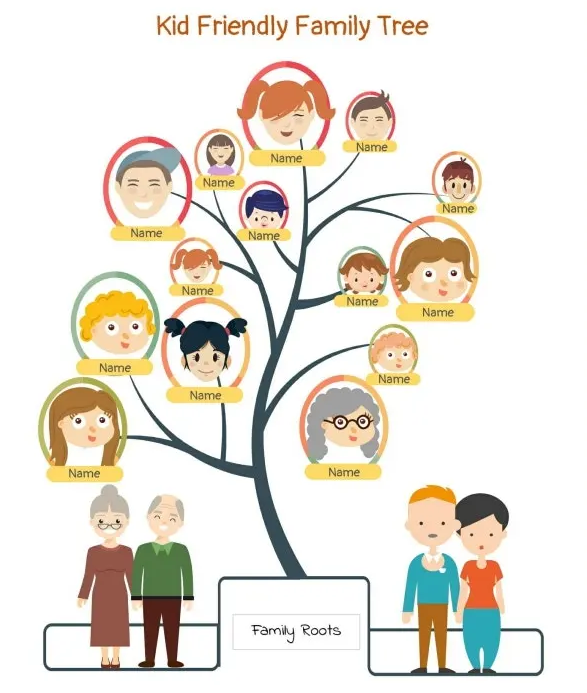
\includegraphics[width= 0.6\linewidth]{tree2}
	\vspace*{-5pt}
\end{figure}